\documentclass[
sigconf, % conference proceedings
%anonymous,  % do not show authors
nonacm,
%authorversion,
%natbib,  % bib style
balance  % equalize columns on last page
]{acmart}

%% The following content must be adapted for the final version
% paper-specific
\newcommand\vldbdoi{XX.XX/XXX.XX}
\newcommand\vldbpages{XXX-XXX}
% issue-specific
\newcommand\vldbvolume{14}
\newcommand\vldbissue{1}
\newcommand\vldbyear{2020}
% should be fine as it is
\newcommand\vldbauthors{\authors}
\newcommand\vldbtitle{\shorttitle}
% leave empty if no availability url should be set
\newcommand\vldbavailabilityurl{https://github.com/vmware/database-stream-processor}
% whether page numbers should be shown or not, use 'plain' for review versions, 'empty' for camera ready
\newcommand\vldbpagestyle{plain}


%\acmConference[CONF]{Conference}{2022}{USA}
%\settopmatter{printfolios=true} % print page numbers

\usepackage{amsmath}
\usepackage{amsfonts}
\usepackage[utf8]{inputenc}
\usepackage{array}
\usepackage{stmaryrd}
\usepackage{tikz}
\usepackage{comment}
\usepackage{xspace}
\usepackage{listofitems}
\usepackage{graphicx}
\usepackage[final]{listings}
\usepackage{hyperref}
\usepackage{enumitem}
\usepackage{amsthm}
%\usepackage{titlesec}
\usepackage{ifthen}

% space saving tricks
\newif\ifstreamexamples
\streamexamplestrue
\newif\ifzsetexamples
\zsetexamplestrue
%\titlespacing{\paragraph}{0pt}{0pt}{1em}
%\titlespacing{\section}{0pt}{*.9}{*.9}
%\titlespacing{\subsection}{0pt}{*.9}{*.9}
\widowpenalty=0
\clubpenalty=0
\newtheoremstyle{note} % name
{2pt} % Space above
{2pt} % Space below
{}    % Body font
{}    % Indent amount
{\bfseries} % Theorem head font
{:}   % Punctuation after theorem head
{.5em}% ⟨Space after theorem head
{}    % Theorem head spec (can be left empty, meaning ‘normal’

\numberwithin{equation}{section}

\graphicspath{ {.} }
\lstset{language=Java,
  commentstyle=\color{brown},
  keywordstyle=\color{blue},
  stringstyle=\color{red},
  basicstyle=\ttfamily}

\lstdefinelanguage{ddlog}{
  language=Java, % we base it on Java, just for comments
  morekeywords={input, output, typedef, relation, typedef, bool, not,
    string, bit, extern, function, var, for, match, skip, in, integer, % not really in DDlog
    Aggregate, FlatMap},
  deletestring=[b]{'}
}
\hypersetup{
  colorlinks   = true,    % Colours links instead of ugly boxes
  urlcolor     = blue,    % Colour for external hyperlinks
  linkcolor    = blue,    % Colour of internal links
  citecolor    = red      % Colour of citations
}
\hypersetup{final}

\usetikzlibrary{shapes, arrows.meta, positioning}
\tikzstyle{block}=[draw,fill=white,rectangle]
\tikzstyle{every node}=[font=\small]

\theoremstyle{note}
\newtheorem{theorem}{Theorem}[section]
\newtheorem{lemma}[theorem]{Lemma}
\newtheorem{corollary}[theorem]{Corollary}
\newtheorem{definition}[theorem]{Definition}
\newtheorem{proposition}[theorem]{Proposition}
\newtheorem{example}[theorem]{Example}
\newtheorem{algorithm}[theorem]{Algorithm}
\newcommand{\dbsp}{DBSP\xspace}

\newcommand{\anonymize}[1]{#1}
% Used when a term is first defined.  Adds the term to the index.
\newcommand{\defined}[1]{\textbf{#1}\index{}}
\newcommand{\zr}{$\Z$-set\xspace}
\newcommand{\zrs}{$\Z$-sets\xspace} % plural
\newcommand{\means}[1]{\ensuremath{\llbracket #1 \rrbracket}}
\newcommand{\code}[1]{\mbox{\texttt{#1}}}
\newcommand{\Z}{\mathbb{Z}}  % integers
\newcommand{\N}{\mathbb{N}}  % naturals
\newcommand{\B}{\mathbb{B}}  % Booleans
\newcommand{\R}{\mathbb{R}}  % reals
% stream with elements of a given type
\newcommand{\stream}[1]{\ensuremath{\mathcal{S}_{#1}}}
% finite stream with elements of a given type (zero almost everywhere)
\newcommand{\streamf}[1]{\ensuremath{\overline{\mathcal{S}_{#1}}}}
\newcommand{\zm}{\ensuremath{z^{-1}}} % stream delay operator
\ifthenelse{\equal{1}{1}}{ % allows switching to mathit/mathcal
\newcommand{\I}{\mathcal{I}}  % stream integration
\newcommand{\D}{\mathcal{D}}  % stream derivative
}{
\newcommand{\I}{\mathit{I}}  % stream integration
\newcommand{\D}{\mathit{D}}  % stream derivative
}
\newcommand{\inc}[1]{{#1}^{\Delta}}
\newcommand{\distinct}{\mathit{distinct}}  % distinct operator
% set with elements of given type
\newcommand{\secref}[1]{\S\ref{#1}}  % reference to a section
\newcommand{\refsec}[1]{\secref{#1}}
\newcommand{\set}[1]{\mathit{set}_{#1}}
\newcommand{\id}{\ensuremath{\mathit{id}}} % identity function
\newcommand{\isset}{\mbox{isset}}
\newcommand{\ispositive}{\mbox{ispositive}}
\newcommand{\defn}{\stackrel{\textrm{\scriptsize def}}{=}}
\newcommand{\map}{\mbox{map}}
\newcommand{\fix}[2]{\mbox{fix}\,#1.#2}
\newcommand{\lift}[1]{{\uparrow}#1}
\newcommand{\rew}{\ensuremath{\mapsto}} % rewriting
\newcommand{\birew}{\ensuremath{\mapsfrom\!\mapsto}} % bidirectional rewriting
\newcommand{\pair}[2]{\ensuremath{\langle #1,#2 \rangle}} % pairing
\newcommand{\norm}[1]{\| #1 \|} % norm; requires math mode
%\newcommand{\zpp}[1]{\mbox{zpp}(#1)}
\newcommand{\makeset}{\ensuremath{\mbox{makeset}}}
\newcommand{\sv}[1]{ % simple stream value, supplied as a space-separated list of 5 values
\setsepchar{ }
\readlist\arg{#1}
{[}
\begin{array}{cccccc}
    \arg[1] & \arg[2] & \arg[3] & \arg[4] & \arg[5] & \cdots
\end{array}
{]}
}

\newcommand{\st}{\;|\;}

\newcommand{\cut}[2]{#1|_{_{\leq #2}}}
\newcommand{\scut}[2]{#1|_{_{< #2}}}

\setlength{\marginparwidth}{1.5cm}
%\newcommand{\scream}[2]{\marginpar{\raggedright \footnotesize \textbf{#1}: #2}}
\newcommand{\scream}[2]{{\color{red} \textbf{#1}: #2}}
\newcommand{\val}[1]{\scream{VAL}{#1}}
\newcommand{\mihai}[1]{\scream{MIHAI}{#1}}
\newcommand{\leonid}[1]{\scream{LEONID}{#1}}
\newcommand{\frank}[1]{\scream{FRANK}{#1}}
\newcommand{\tej}[1]{\scream{TEJ}{#1}}

\title{\dbsp: Automatic Incremental View Maintenance for Rich Query Languages}
\author{Mihai Budiu}
\affiliation{VMware Research}
\email{mbudiu@vmware.com}

\author
{Tej Chajed}
\affiliation{VMware Research}
\email{tchajed@vmware.com}

\author
{Frank McSherry}
\affiliation{Materialize Inc.}
\email{mcsherry@materialize.com}

\author
{Leonid Ryzhyk}
\affiliation{VMware Research}
\email{lryzhyk@vmware.com}

\author
{Val Tannen}
\affiliation{University of Pennsylvania}
\email{val@seas.upenn.edu}

\begin{abstract}
Incremental view maintenance (IVM) has long been a central problem in
database theory.  Many solutions have been proposed for restricted
classes of database languages, such as the relational algebra, or
Datalog.  These techniques do not naturally generalize to richer
languages.  In this paper we give a general, heuristic-free solution
to this problem in 3 steps: (1) we describe a simple but expressive
language called \dbsp for describing computations over data streams;
(2) we give a new mathematical definition of IVM and a general
algorithm for solving IVM for arbitrary \dbsp programs, and (3) we
show how to model many rich database query languages using \dbsp
(including the full relational algebra, queries over sets and
multisets, arbitrarily nested relations, aggregation, flatmap
(unnest), monotonic and non-monotonic recursion, streaming
aggregation, and arbitrary compositions of all of these).  SQL and
Datalog can both be implemented in \dbsp.  As a consequence, we
obtain efficient incremental view maintenance algorithms for queries
written in all these languages.
\end{abstract}

\begin{document}

\maketitle

\pagestyle{\vldbpagestyle}
\begingroup\small\noindent\raggedright\textbf{PVLDB Reference Format:}\\
\vldbauthors. \vldbtitle. PVLDB, \vldbvolume(\vldbissue): \vldbpages, \vldbyear.\\
\href{https://doi.org/\vldbdoi}{doi:\vldbdoi}
\endgroup
\begingroup
\renewcommand\thefootnote{}\footnote{\noindent
This work is licensed under the Creative Commons BY-NC-ND 4.0 International License. Visit \url{https://creativecommons.org/licenses/by-nc-nd/4.0/} to view a copy of this license. For any use beyond those covered by this license, obtain permission by emailing \href{mailto:info@vldb.org}{info@vldb.org}. Copyright is held by the owner/author(s). Publication rights licensed to the VLDB Endowment. \\
\raggedright Proceedings of the VLDB Endowment, Vol. \vldbvolume, No. \vldbissue\ %
ISSN 2150-8097. \\
\href{https://doi.org/\vldbdoi}{doi:\vldbdoi} \\
}\addtocounter{footnote}{-1}\endgroup
%%% VLDB block end %%%

%%% do not modify the following VLDB block %%
%%% VLDB block start %%%
\ifdefempty{\vldbavailabilityurl}{}{
\vspace{.3cm}
\begingroup\small\noindent\raggedright\textbf{PVLDB Artifact Availability:}\\
The source code, data, and/or other artifacts have been made available at \url{\vldbavailabilityurl}.
\endgroup
}
%%% VLDB block end %%%


\section{Introduction}\label{sec:introduction}

Incremental view maintenance (IVM) is an important and well-studied problem in
databases~\cite{gupta-idb95}.  The IVM problem can be stated as follows: given a database $DB$ and
a view $V$ described by a query $Q$ that is a function of the database, i.e. $V = Q(DB)$,
maintain the contents of $V$ in response to changes of the database,
ideally more efficiently than by simply reevaluating $Q(DB)$ from scratch.  The goal is
to provide an algorithm that can evaluate $Q$ over the changes $\Delta DB$ applied
to the database, since in general the size of the changes is small $|\Delta DB| \ll |DB|$.

This paper provides a new perspective by proposing a new definition
of IVM based on a streaming model of computation\footnote{Our model is inspired by Digital Signal
Processing DSP~\cite{rabiner-book75}, applied to databases, hence the name \dbsp.}.  Whereas previous
IVM solutions are based on defining a notion of a (partial) derivative of $Q$ with respect to its inputs,
our definition only requires computing \emph{derivatives of streams} as functions of time.
Derivatives of streams are always well-defined if the data computed on has a notion of difference
that satisfies some simple mathematical properties --- specifically, that it forms a commutative
group.  (Fortunately, it has long been known that relational databases can be modeled
in such a way, e.g.~\cite{green-pods07, koch-pods10}.)

\dbsp has several attractive properties:

\begin{enumerate}[nosep, leftmargin=0pt, itemindent=0.5cm, label=\textbf{(\arabic{*})}]
\item it is \textbf{expressive}.  (a) It can be used to define
precisely multiple concepts: traditional queries, streaming computations, and incremental
computations.  (b) We have been able to express in \dbsp the full
relational algebra, computations over sets and bags,
nested relations, aggregation, flatmap, monotonic and nonmonotonic
recursion, stratified negation, while-relational programs, window queries,
streaming queries, streaming aggregation, and incremental versions of all
of the above.  In fact, we have built a \dbsp implementation of the
complete SQL language (\refsec{sec:implementation}).
\item it is \textbf{simple}.
\dbsp is built entirely on elementary concepts such as functions and algebraic groups.
\item mathematically \textbf{precise}.  All the results in this paper have been
formalized and checked using the Lean
proof assistant~\cite{moura-cade15}.
\item it is \textbf{modular}, in the following sense:
(a) the incremental version of a complex query can be reduced
recursively to incrementalizing its component subqueries.
This gives a simple, syntactic,
heuristic-free algorithm (Algorithm~\ref{algorithm-inc})
that converts an arbitrary \dbsp query plan to its incremental form.
(b) Extending \dbsp to support new primitive operators is easy,
and they immediately benefit from the rest of the theory of
incrementalization.
An important consequence of modularity is that the theory
can be efficiently implemented, as we
briefly discuss in \refsec{sec:implementation}.
\end{enumerate}

The core concept of \dbsp is the \emph{stream}, which is used to model changes
over time. We use $\stream{A}$ to denote the type of infinite streams with values of
type $A$. If $s \in \stream{A}$ is a stream,
then $s[t] \in A, t \in \mathbb{N}$ is the $t$-th element of $s$, also referred to as the \emph{value of the stream at time $t$}.
A streaming operator is a function that
consumes one or more streams and produces another stream.  We show
streaming computations with diagrams, also called ``circuits'',
where boxes are computations and streams are arrows.  The following diagram
shows a stream operator $T: \stream{A} \times \stream{B} \to \stream{C}$,
consuming two input streams $s_0$ and $s_1$
and producing one output stream $s$:

\begin{center}
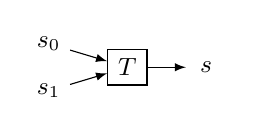
\begin{tikzpicture}[auto,>=latex,minimum width=.5cm]
  \node[] (input0) {$s_0$};
  \node[below of=input0,node distance=.3cm] (dummy) {};
  \node[below of=dummy,node distance=.3cm] (input1) {$s_1$};
  \node[block, right of=dummy] (T) {$T$};
  \node[right of=T] (output) {$s$};
  \draw[->] (input0) -- (T);
  \draw[->] (input1) -- (T);
  \draw[->] (T) -- (output);
\end{tikzpicture}
\vspace{-.2cm}
\end{center}

We generally think of streams as sequences of ``small'' values,
such as insertions or deletions in a database.
However, we also treat the whole database as a \emph{stream of database
snapshots}.  We model a database as a
stream $DB \in \stream{SCH}$, where $SCH$ is the database schema.
Time is not wall-clock time, but counts
the transactions applied to the database.
Since transactions are linearizable, they have a total order.
$DB[t]$ is the snapshot of the
database contents after $t$ transactions have been applied.

Database transactions also form a stream $\Delta DB$, this time a stream of \emph{changes},
or \emph{deltas} that are applied to the database.  The values of
this stream are defined by $(\Delta DB)[t] = DB[t] - DB[t-1]$, where ``$-$'' stands
for the difference between two databases, a notion that we will soon make more precise.
The $\Delta DB$ stream is produced from the $DB$ stream by
the \emph{stream differentiation} operator $\D$;
this operator produces as its output the stream of changes from its input stream;
we have thus $\D(DB) = \Delta DB$.

Conversely, the database snapshot at time $t$ is the cumulative result of applying all
transactions up to $t$: $DB[t] = \sum_{i \leq t} \Delta DB[i]$.
The operation of adding up all changes is the inverse of differentiation,
and is another basic stream operator, \emph{stream integration}: $\I$.
The following diagram expresses the relationship between the streams $\Delta DB$ and $DB$:

\begin{center}
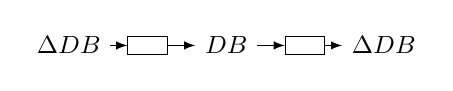
\begin{tikzpicture}[auto,>=latex,minimum width=.5cm]
  \node[] (input) {$\Delta DB$};
  \node[block, right of=input] (I) {$\I$};
  \node[right of=I] (output) {$DB$};
  \node[block, right of=output] (D) {$\D$};
  \node[right of=D] (end) {$\Delta DB$};
  \draw[->] (input) -- (I);
  \draw[->] (I) -- (output);
  \draw[->] (output) -- (D);
  \draw[->] (D) -- (end);
\end{tikzpicture}
\end{center}

Suppose we have a query $Q : SCH \to SCH$ defining a view $V$.  What is
a view in a streaming model?  It is also a stream!  For each snapshot
of the database stream we have a snapshot of the view: $V[t] = Q(DB[t])$.
In general, given an arbitrary function $f: A \to B$, we define
a streaming ``version'' of $f$, denoted by $\lift{f}$
(read as ``$f$ lifted''), which applies
$f$ to every element of the input stream independently.
We can thus write $V = (\lift{Q})(DB)$.

Armed with these basic definitions, we can now precisely define IVM.
What does it mean to maintain a view incrementally?  We claim that an
efficient maintenance algorithm needs to compute the \emph{changes} to
the view given the changes to the database. Given a query $Q$, a key
contribution of this paper is the definition of its \emph{incremental
  version} $\inc{Q}$ that uses stream integration and differentiation:
$\inc{Q} \defn D \circ \lift Q \circ I$. The incremental version of
the query maintains the changes to the view $\Delta V \defn \D(V) =
\D(\lift{Q}(\I(\Delta DB)))$, depicted graphically as:

\begin{center}
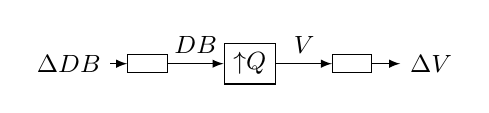
\begin{tikzpicture}[auto,>=latex,minimum width=.5cm]
  \node[] (input) {$\Delta DB$};
  \node[block, right of=input] (I) {$\I$};
  \node[block, right of=I, node distance=1.3cm] (Q) {$\lift{Q}$};
  \node[block, right of=Q, node distance=1.3cm] (D) {$\D$};
  \node[right of=D] (output) {$\Delta V$};
  \draw[->] (input) -- (I);
  \draw[->] (I) -- node (db) {$DB$} (Q);
  \draw[->] (Q) -- node (B) {$V$} (D);
  \draw[->] (D) -- (output);
\end{tikzpicture}
\end{center}

The incremental version of a query is a \emph{streaming operator}
which computes directly on changes and produces changes.  The
incremental version of a query is thus always well-defined.  The above
definition shows one way to compute a query incrementally, but
applying it naively produces an inefficient execution plan, since it
will reconstruct the database at each step.  In
\refsec{sec:incremental} we show how algebraic properties of the
$\inc{\cdot}$ transformation can be used to optimize the
implementation of $\inc{Q}$. The first key property is that the
composition of queries can be incrementalized by composing the
incremental versions of its constituents, that is $\inc{(Q_1 \circ
  Q_2)} = \inc{Q_1} \circ \inc{Q_2}$.  The second key property is that
essentially all primitive database operations have efficient
incremental versions\footnote{They are faster than non-incremental
versions by a factor of $O(|DB|/|\Delta DB|)$.}.

Armed with this general theory of incremental computation, in
\secref{sec:relational} we show how to model relational queries in
\dbsp.  This immediately gives us a general algorithm to compute the
incremental version of any relational query.  These results were
previously known, but they are cleanly modeled by \dbsp.
\secref{sec:datalog} shows how stratified-monotonic recursive Datalog
programs can be implemented in \dbsp, and \secref{sec:nested} gives
\emph{incremental streaming computations for recursive programs}. For
example, given an implementation of transitive closure in the natural
recursive way, our algorithm produces a program that efficiently
maintains the transitive closure of a graph as the graph is changed by
adding and deleting edges.

Due to space reasons, this paper omits proofs.  A companion extensive
technical report\anonymize{~\cite{tr}} contains the proofs.  We have
formalized the entire \dbsp theory in the Lean proof
assistant~\anonymize{\cite{dbsp-theory}}; our formalization includes
machine-checked proofs of correctness for all the theorems stated in
this paper.

This paper makes the following contributions:
\begin{enumerate}[nosep, leftmargin=0pt, itemindent=0.5cm, label=\textbf{(\arabic{*})}]
  \item \dbsp, a \textbf{simple} but \textbf{expressive} language for streaming
  computation. \dbsp gives an elegant formal foundation unifying the manipulation of
  streaming and incremental computations.
  \item An algorithm for incrementalizing any streaming computation expressed in
  \dbsp.
  \item An illustration of how \dbsp can model various query classes, such as relational algebra,
  nested relations, aggregations, flatmap, and stratified-monotonic Datalog.
  \item The first general and machine-checked theory of IVM.
  \item A high-performance open-source implementation of DBSP as a
  general-purpose streaming query engine in Rust.
\end{enumerate}

\section{Stream computations}\label{sec:streams}

The core notion of our theory of IVM is the \textbf{stream}.
In this section we introduce formally streams as a
infinite sequences of values, and define computations on streams.
Stream operators (\secref{sec:notation}) are the basic building block of stream
computations.  Operators can be composed with simple rules (\secref{sec:abelian})
into complex computational circuits.
In (\secref{sec:abelianstreams}) we introduce two essential operations on streams:
integration and differentiation.

\subsection{Streams and stream operators}\label{sec:notation}

$\N$ is the set of natural numbers (from 0), $\B$ is the set of
Booleans, $\Z$ is the set of integers, and $\R$ is the set of real
numbers.

\begin{definition}[stream]
Given a set $A$, a \defined{stream} \emph{of values from $A$}, or an
\emph{$A$-stream}, is a function $\N \rightarrow A$.  We denote by
$\stream{A} \defn \{ s \,|\, s : \N \to A \}$ the set of all
$A$-streams.
\end{definition}

When $s\in\stream{A}$ and $t\in\N$ we
write $s[t]$ for the $t$-th element of the stream $s$ instead of the usual $s(t)$
to distinguish it from other function applications.
We think of the index $t\in\N$ as (discrete) time and of $s[t]\in A$
as the value of the the stream $s$ ``at time'' $t$.
\ifstreamexamples
For example, the stream of natural numbers $id \in \stream{\N}$ given by $\id[t] = t$ is the sequence of values
$\sv{0 1 2 3 4}$.
\fi

\begin{definition}[stream operator]
A \defined{stream operator} with $n$ inputs is a function
$T:\stream{A_0}\times\cdots\times\stream{A_{n-1}}\to\stream{B}$.
\end{definition}

In general we use ``operator'' for functions on streams, and
``function'' for computations on ``scalar'' values.

DBSP is an extension of the simply-typed lambda calculus ---
we will introduce its elements gradually.  However, in many cases we find it more readable to
use circuit diagrams to depict \dbsp programs
\footnote{Circuits however hide the \emph{order} of the inputs of an operator; for non-commutative
operators we have to label the operator inputs.}.
In a circuit a rectangle represents an operator application (labeled
with the operator name, e.g., $T$), while an arrow is a stream.

Stream operator \emph{composition} (function composition) is shown as chained circuits.
The composition of a binary operator $T: \stream{A} \times \stream{B} \to \stream{A}$ with the
unary operator $S: \stream{A} \to \stream{B}$ into the computation
$\lambda s. T(T(s,S(s)),S(s)) : \stream{A}\to\stream{A}$
is:

\begin{center}
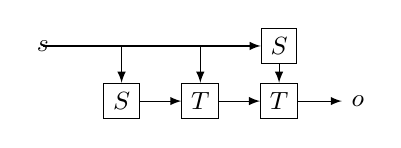
\begin{tikzpicture}[auto,>=latex]
  \node[] (input) {$s$};
  \node[] [right of=input] (dummy) {};
  \node[block, below of=dummy, node distance=.7cm] (S1) {$S$};
  \node[block, right of=S1] (T1) {$T$};
  \node[block, right of=T1] (T2) {$T$};
  \node[block, above of=T2, node distance=.7cm] (S2) {$S$};
  \node[right of=T2] (output) {$o$};
  \draw[->] (input) -| (S1);
  \draw[->] (input) -| (T1);
  \draw[->] (S1) -- (T1);
  \draw[->] (T1) -- (T2);
  \draw[->] (input) |- (S2);  \draw[->] (T2) -- (output);
  \draw[->] (S2) -- (T2);
\end{tikzpicture}
\end{center}


\begin{definition}(lifting)
Given a (scalar) function $f: A \to B$,
we define a stream operator $\lift{f} :\stream{A} \to \stream{B}$
by \emph{lifting} the function $f$ pointwise in time: $(\lift{f})(s) \defn f \circ s$.
Equivalently, $((\lift{f})(s))[t] \defn f(s[t])$.
This extends to functions of multiple arguments.
\end{definition}

\ifstreamexamples
For example, $(\lift{(\lambda x.(2x))})(id) = \sv{0 2 4 6 8}$.
\fi

\begin{proposition}[distributivity]\label{prop:distributivity}
Lifting distributes over function composition:
$\lift{(f \circ g)} = (\lift{f}) \circ (\lift{g})$.
\end{proposition}
\begin{comment}
\begin{proof}
This is easily proved by using associativity of function composition:
$\forall s . (\lift{(f \circ g)})(s) = (f \circ g) \circ s =
f \circ (g \circ s) = f \circ (\lift{g})(s) = (\lift{f})((\lift{g})(s)) =
(\lift{f} \circ \lift{g})(s).$
\end{proof}
\end{comment}

We say that two \dbsp programs are \defined{equivalent} if they compute the same
input-output function on streams.
We use the symbol $\cong$ to indicate that two circuits are
equivalent.  For example, Proposition~\ref{prop:distributivity}
states the following circuit equivalence:

\noindent
\begin{tabular}{m{3.5cm}m{.3cm}m{3.5cm}}
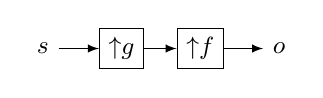
\begin{tikzpicture}[auto,>=latex]
  \node[] (input) {$s$};
  \node[block, right of=input] (g) {$\lift{g}$};
  \node[block, right of=g] (f) {$\lift{f}$};
  \node[right of=f] (output) {$o$};
  \draw[->] (input) -- (g);
  \draw[->] (g) -- (f);
  \draw[->] (f) -- (output);
\end{tikzpicture}
&
$\cong$
&
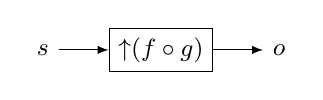
\begin{tikzpicture}[auto,>=latex]
    \node[] (input) {$s$};
    \node[block, right of=input, node distance=1.5cm] (fg) {$\lift{(f \circ g)}$};
    \node[right of=fg, node distance=1.5cm] (output) {$o$};
    \draw[->] (input) -- (fg);
    \draw[->] (fg) -- (output);
\end{tikzpicture}
\end{tabular}

\subsection{Streams over abelian groups}\label{sec:abelian}

For the rest of the technical development we require the set of values $A$
of a stream $\stream{A}$ to form a commutative group $(A, +, 0_A, -)$.
We show later that this restriction is not a problem
for using \dbsp with relational data.
Now we introduce some useful operators and study their properties.

\subsubsection{Delays and time-invariance}\label{sec:delay}

\begin{definition}[Delay]
The \defined{delay operator}\footnote{The name $\zm$
comes from the DSP literature, and is related to the z-transform~\cite{rabiner-book75}.}
produces an output stream
by delaying its input by one step: $\zm_A: \stream{A} \to \stream{A}$:
%\begin{tabular}{m{5cm}m{3cm}}
$$
\zm_A(s)[t] \defn   \begin{cases}
0_A      & \text{when}~t=0 \\
s[t - 1] & \text{when}~t\geq1
\end{cases}
$$
%&
%\begin{tikzpicture}[auto,node distance=1cm,>=latex]
%    \node[] (input) {$s$};
%    \node[block, right of=input] (z) {$\zm$};
%    \node[right of=z] (output) {$o$};
%    \draw[->] (input) -- (z);
%    \draw[->] (z) -- (output);
%\end{tikzpicture}
%\end{tabular}
\end{definition}

We often omit the type parameter $A$, and write just $\zm$.
\ifstreamexamples
For example, $\zm(\id) = \sv{0 0 1 2 3}$.
\fi

\begin{definition}[Time invariance]
A stream operator $S: \stream{A} \to \stream{B}$ is \defined{time-invariant} (TI) if
$S(\zm_A(s)) = \zm_B(S(s))$ for all $s \in \stream{A}$, or, in other words, if the
following two circuits are equivalent:

\begin{tabular}{m{3cm}m{.5cm}m{3cm}}
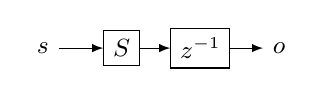
\begin{tikzpicture}[auto,>=latex]
  \node[] (input) {$s$};
  \node[block, right of=input] (S) {$S$};
  \node[block, right of=S] (z) {$\zm$};
  \node[right of=z] (output) {$o$};
  \draw[->] (input) -- (S);
  \draw[->] (S) -- (z);
  \draw[->] (z) -- (output);
\end{tikzpicture}
&
$\cong$
&
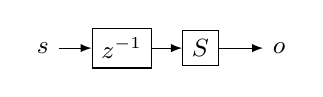
\begin{tikzpicture}[auto,>=latex]
  \node[] (input) {$s$};
  \node[block, right of=input] (z) {$\zm$};
  \node[block, right of=z] (S) {$S$};
  \node[right of=S] (output) {$o$};
  \draw[->] (input) -- (z);
  \draw[->] (z) -- (S);
  \draw[->] (S) -- (output);
\end{tikzpicture}
\end{tabular}

\noindent
This definition extends
naturally to operators with multiple inputs.
\end{definition}

The composition of TI operators of any number of inputs
is TI. The delay operator $\zm$ is TI.
\dbsp only uses TI operators.

%\begin{definition}
%We say that a function between groups $f: A \to B$ has the \emph{zero-preservation
%property} if $f(0_A) = 0_B$.  We write $\zpp{f}$.
%\end{definition}
%
%A lifted operator $\lift{f}$ is TI iff $\zpp{f}$.

\subsubsection{Causal and strict operators}\label{sec:causal}

\begin{definition}[Causality]
A stream operator $S:\stream{A}\to\stream{B}$
is \defined{causal} when for all $s,s'\in\stream{A}$,
and all times $t$ we have:
$
(\forall i \leq . t~s[i]=s'[i]) ~~\Rightarrow~~ S(s)[t]=S(s')[t].
$
\end{definition}

\noindent
In other words, the output value at time $t$ can only depend on
input values from times $t' \leq t$.
Operators produced by lifting are causal, and $\zm$ is causal.
All \dbsp operators are causal.  The composition
of causal operators of any number of inputs is causal.

\begin{definition}[Strictness]
A stream operator, $F:\stream{A}\to\stream{B}$
is \defined{strict}
if  $\forall s,s'\in\stream{A}, \forall t \in \N$ we have:
$(\forall i<t . ~s[i]=s'[i]) ~~\Rightarrow \\ F(s)[t]=F(s')[t].$
\end{definition}

In other words, the $t$-th output of $F(s)$ can depend only on ``past'' values
of the input $s$, between $0$ and $t-1$.
In particular, $F(s)[0] = 0_B$ is the same for all $s \in \stream{A}$.
Strict operators are causal. Lifted operators in general are \emph{not} strict.
$\zm$ is strict.  %In \dbsp $\zm$ is the only primitive strict operator.

\begin{proposition}
\label{prop-unique-fix}
For a strict $F: \stream{A} \to \stream{A}$ the equation ~$\alpha=F(\alpha)$~ has a unique
solution $\alpha \in \stream{A}$, denoted by $\fix{\alpha}{F(\alpha)}$.
\end{proposition}

Thus every strict operator from a set to itself has a unique fixed point.
The simple proof relies on strong induction, showing that $\alpha[t]$
depends only on the values of $\alpha$ prior to $t$.

The next lemma show that the following circuit, having a strict
``feedback'' edge $F$, is a well-defined function on streams:
\begin{center}
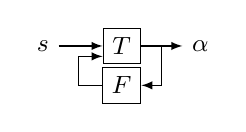
\begin{tikzpicture}[>=latex]
    \node[] (input) {$s$};
    \node[block, right of=input] (f) {$T$};
    \node[right of=f] (output) {$\alpha$};
    \node[block, below of=f, node distance=.5cm] (z) {$F$};
    \draw[->] (input) -- (f);
    \draw[->] (f) -- node (mid) {} (output);
    \draw[->] (mid.center) |-  (z);
    \draw[->] (z.west) -- ++(-.3,0) |- ([yshift=1mm]f.south west);
\end{tikzpicture}
\end{center}

%\begin{lemma}
%\label{lemma-causal-strict}
%If $F: \stream{B} \to \stream{B}$ is strict and $T: \stream{A} \times \stream{B} \to \stream{B}$ is causal, then for fixed $s$ the operator
%$\lambda\alpha.T(s,F(\alpha)): \stream{A} \to \stream{B}$ is strict.
%\end{lemma}

\begin{lemma}\label{feedback-semantics}
\label{cor-loop}
If $F: \stream{B} \to \stream{B}$ is strict and $T: \stream{A} \times \stream{B} \to \stream{B}$ is causal,
the operator $Q(s)=\fix{\alpha}{T(s,F(\alpha))}$ is well-defined and causal.
If, moreover, $F$ and $T$ are TI then so is $Q$.
\end{lemma}

All stream computations in \dbsp are built from the primitive operators
we have described: lifted operators and delays (we add two more operators in \secref{sec:nested}).
%Circuits composed of such operators can be efficiently implemented
%using Dataflow machines~\cite{lee-ieee95}.

%Circuits with feedback are used for two purposes: defining an
%integration operator (in the next section), and defining recursive computations (\secref{sec:recursion}).  In turn, the
%integration operator will be instrumental in defining incremental
%computations (\secref{sec:incremental}).

\subsection{Integration and differentiation}\label{sec:abelianstreams}

Remember that we require the elements of a stream to come from an abelian group $A$.
Streams themselves form an abelian group:

\begin{proposition}
The structure $(\stream{A},+,0,-)$, obtained by lifting the $+$ and unary $-$ operations of $A$,
is an abelian group.  0 is the stream with all values $0_A$.
\end{proposition}

\noindent
Stream addition and negation are causal, TI operators.

\begin{definition}
Given abelian groups $A$ and $B$ we call a stream operator
$S: \stream{A} \rightarrow \stream{B}$ \defined{linear} if it is a group homomorphism, that is,
$S(a+b)=S(a)+S(b)$ (and therefore $S(0)=0$ and $S(-a)=-S(a)$).
\end{definition}

Lifting a linear function $f: A \to B$ produces
a stream operator $\lift{f}$ that is linear and TI (LTI).
$\zm$ is also LTI.

\begin{definition}(bilinear)
A function of two arguments $f: A \times B \to C$ with $A, B, C$ groups, is \emph{bilinear}
if it is linear separately in each argument (i.e., it distributes over addition):
$\forall a, b, c, d . f(a+b, c) = f(a, c) + f(b, c)$, and $f(a, c+d) = f(a, c) + f(c, d).$
\end{definition}

This definition extends to stream operators.
Lifting a bilinear function $f: A \times B \to C$ produces
a bilinear stream operator $\lift{f}$.  An example bilinear operator over $\stream{\Z}$
is lifted multiplication:
$f: \stream{\N} \times \stream{\N} \to \stream{\N}, f(a, b)[t] = a[t]\cdot b[t]$.

%The composition of (bi)linear operators with linear operators
%is (bi)linear (since homomorphisms compose).

The ``feedback loop'' of a linear operator is linear:

\begin{proposition}
\label{prop-rec-linear}
Let $S$ be a unary causal LTI operator. The
operator $Q(s)=\fix{\alpha}{S(s+\zm(\alpha))}$ is well-defined and LTI:

\begin{center}
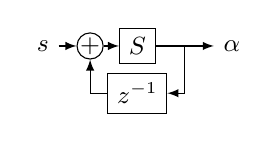
\begin{tikzpicture}[>=latex]
    \node[] (input) {$s$};
    \node[block, shape=circle, right of=input, inner sep=0pt, node distance=.6cm] (plus) {$+$};
    \node[block, right of=plus, node distance=.6cm] (Q) {$S$};
    \node[right of=Q, node distance=1.2cm] (output) {$\alpha$};
    \node[block, below of=Q, node distance=.6cm] (z) {$\zm$};
    \draw[->] (input) -- (plus);
    \draw[->] (plus) -- (Q);
    \draw[->] (Q) -- node (mid) {} (output);
    \draw[->] (mid.center) |-  (z);
    \draw[->] (z) -| (plus);
\end{tikzpicture}
\end{center}
\end{proposition}

\begin{definition}[Differentiation]
The \defined{differentiation operator} $\D_{\stream{A}} : \stream{A} \to \stream{A}$ is defined by:
$\D(s) \defn s - \zm(s)$.

\begin{center}
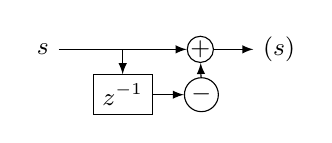
\begin{tikzpicture}[auto,>=latex,node distance=1cm]
    \node[] (input) {$s$};
    \node[block, shape=circle, right of=input, inner sep=0pt,node distance=2cm] (plus) {$+$};
    \node[right of=plus] (output) {$\D(s)$};
    \draw[draw,->] (input) -- node (i) {} (plus);
    \node[block, below of=i, node distance=.7cm] (z) {$\zm$};
    \node[block, shape=circle, right of=z, inner sep=1pt] (minus) {$-$};
    \draw[->] (plus) -- (output);
    \draw[->] (i) -- (z);
    \draw[->] (z) -- (minus);
    \draw[->] (minus) -- (plus);
\end{tikzpicture}
\end{center}
\end{definition}
We generally omit the type, and write just $\D$.
The value of $\D(s)[t] = s[t] - s[t-1]$ if $t > 0$.
\ifstreamexamples
As an example, $\D(\id) = \sv{0 1 1 1 1}$.
\fi

If $s$ is a stream, then $\D(s)$ is the \emph{stream of changes} of $s$.

\begin{proposition}
\label{prop-diff-properties}
$\D$ is causal and LTI.
\end{proposition}

The integration operator ``reconstitutes'' a stream from its changes:

\begin{definition}[Integration]
The \defined{integration operator}  $\I_{\stream{A}} : \stream{A} \to \stream{A}$
is defined by $\I(s) \defn \lambda s . \fix{\alpha}{(s + \zm(\alpha))}$:
\begin{center}
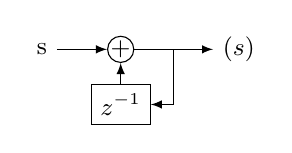
\begin{tikzpicture}[auto,>=latex]
    \node[] (input) {s};
    \node[block, shape=circle, right of=input, inner sep=0pt] (plus) {$+$};
    \node[right of=plus, node distance=1.5cm] (output) {$\I(s)$};
    \node[block, below of=plus, node distance=.7cm] (z) {$z^{-1}$};
    \draw[->] (input) -- (plus);
    \draw[->] (plus) -- node (o) {} (output);
    \draw[->] (o) |- (z);
    \draw[->] (z) -- (plus);
\end{tikzpicture}
\end{center}
\end{definition}

\noindent
We also generally omit the type, and write just $\I$.
This is the construction from Proposition~\ref{prop-rec-linear}
using the identity function for $S$.

\begin{proposition}
$\I(s)$ is the discrete (indefinite) integral applied to the stream $s$:
$\I(s)[t] = \sum_{i \leq t} s[i]$.
\end{proposition}
\ifstreamexamples
As an example, $\I(\id) = \sv{0 1 3 6 10}$.
\fi

\begin{proposition}
\label{prop-integ-properties}
$\I$ is causal and LTI.
\end{proposition}

\begin{theorem}[Inversion]
\label{inverses}
Integration and differentiation are inverses of each other:
$\forall s . \I(\D(s)) = \D(\I(s)) = s$.
\end{theorem}

\noindent
\begin{tabular}{m{2.5cm}m{.3cm}m{1cm}m{.3cm}m{2.5cm}}
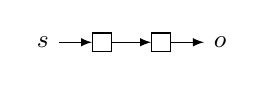
\begin{tikzpicture}[auto,>=latex, node distance=.75cm]
    \node[] (input) {$s$};
    \node[block, right of=input] (I) {$\I$};
    \node[block, right of=I] (D) {$\D$};
    \node[right of=D] (output) {$o$};
    \draw[->] (input) -- (I);
    \draw[->] (I) -- (D);
    \draw[->] (D) -- (output);
\end{tikzpicture}
     &
     $\cong$
     &
     \hspace{-2ex}
\begin{tikzpicture}[auto,>=latex, node distance=.75cm]
    \node[] (input) {$s$};
    \node[right of=input] (output) {$o$};
    \draw[->] (input) -- (output);
\end{tikzpicture}
     &
     $\cong$
     &
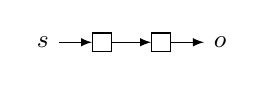
\begin{tikzpicture}[auto,>=latex, node distance=.75cm]
    \node[] (input) {$s$};
    \node[block, right of=input] (D) {$\D$};
    \node[block, right of=D] (I) {$\I$};
    \node[right of=I] (output) {$o$};
    \draw[->] (input) -- (D);
    \draw[->] (D) -- (I);
    \draw[->] (I) -- (output);
\end{tikzpicture}
\end{tabular}

\section{Incremental view maintenance}\label{sec:incremental}

In this section we give a precise definition of IVM and analyze its properties.

\begin{definition}
Given a unary stream operator $Q: \stream{A} \to \stream{B}$ we define the
\defined{incremental version} of $Q$ as:
\begin{equation}\label{def:inc}
\inc{Q} \defn \D \circ Q \circ \I.
\end{equation}
$\inc{Q}$ has the same ``type'' as $Q$: $\inc{Q}: \stream{A} \to \stream{B}$.
For an operator with multiple inputs we define
the incremental version by applying $\I$ to each input independently:
e.g., if $T: \stream{A} \times \stream{B} \rightarrow \stream{C}$ then
$\inc{T}(a, b) \defn \D (T(\I(a), \I(b)))$.
\end{definition}

The following diagram illustrates the intuition behind this definition:
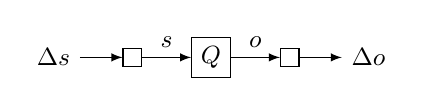
\begin{tikzpicture}[auto,>=latex]
    \node[] (input) {$\Delta s$};
    \node[block, right of=input] (I) {$\I$};
    \node[block, right of=I] (Q) {$Q$};
    \node[block, right of=Q] (D) {$\D$};
    \node[right of=D] (output) {$\Delta o$};
    \draw[->] (input) -- (I);
    \draw[->] (I) -- node (s) {$s$} (Q);
    \draw[->] (Q) -- node (o) {$o$} (D);
    \draw[->] (D) -- (output);
\end{tikzpicture}

If $Q(s) = o$ is a computation, then $\inc{Q}$ performs
the ``same'' computation as $Q$,
but between streams of changes $\Delta s$ and $\Delta o$.

Notice that our definition of incremental computation is meaningful only for \emph{streaming}
computations; this is in contrast to classic definitions, e.g.~\cite{gupta-idb95} which
consider only one change.  Generalizing the definition to operate on streams gives us
additional power, especially when operating with recursive queries.

The following proposition is one of our central results.

\begin{proposition}(Properties of the incremental version):
For computations of appropriate types, the following hold:
\label{prop-inc-properties}
\begin{description}[nosep, leftmargin=\parindent]
\item[inversion:] $Q\mapsto\inc{Q}$ is bijective; its inverse is $Q\mapsto \I\circ Q\circ\D$.
\item[invariance:] $\inc{+} = +, \inc{(\zm)} = \zm, \inc{-} = -, \inc{\I}=\I, \inc{\D}=\D$
\item[push/pull:] \label{prop-part-commutation}
    $Q \circ \I = \I \circ \inc{Q}$; $\D\circ Q = \inc{Q}\circ\D$
\item[chain:] $\inc{(Q_1\circ Q_2)} = \inc{Q_1}\circ\inc{Q_2}$ (This generalizes to operators with multiple inputs.)
\item[add:] $\inc{(Q_1 + Q_2)} = \inc{Q_1} + \inc{Q_2}$
\item[cycle:] $\inc{(\lambda s. \fix{\alpha}{T(s,\zm(\alpha)}))} = \lambda s. \fix{\alpha}{\inc{T}(s,\zm(\alpha)})$
\end{description}
\end{proposition}

These properties are very useful; for example, the \defined{chain rule}  states
that the following two circuits are equivalent:

\noindent
\begin{tabular}{m{4cm}m{.2cm}m{2.5cm}}
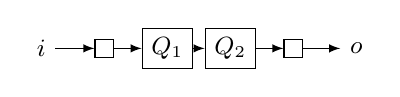
\begin{tikzpicture}[auto,>=latex,node distance=.8cm]
  \node[] (input) {$i$};
  \node[block, right of=input] (I) {$\I$};
  \node[block, right of=I] (Q1) {$Q_1$};
  \node[block, right of=Q1] (Q2) {$Q_2$};
  \node[block, right of=Q2] (D) {$\D$};
  \node[right of=D] (output)  {$o$};
  \draw[->] (input) -- (I);
  \draw[->] (I) -- (Q1);
  \draw[->] (Q1) -- (Q2);
  \draw[->] (Q2) -- (D);
  \draw[->] (D) -- (output);
\end{tikzpicture} &
$\cong$ &
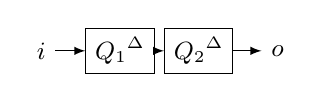
\begin{tikzpicture}[>=latex]
  \node[] (input) {$i$};
  \node[block, right of=input] (Q1) {$\inc{Q_1}$};
  \node[block, right of=Q1] (Q2) {$\inc{Q_2}$};
  \node[right of=Q2] (output)  {$o$};
  \draw[->] (input) -- (Q1);
  \draw[->] (Q1) -- (Q2);
  \draw[->] (Q2) -- (output);
\end{tikzpicture}
\end{tabular}

\noindent In other words, \textbf{to incrementalize a composite query you can incrementalize
each sub-query independently}.  This gives us a simple, syntax-directed, deterministic recipe
for computing the incremental version of an arbitrarily complex query.

The \defined{cycle rule} states that the following circuits are equivalent:

\noindent
\begin{tabular}{m{4.2cm}m{.2cm}m{3cm}}
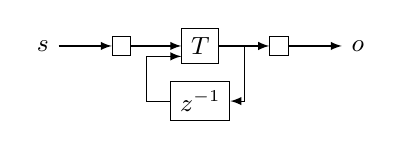
\begin{tikzpicture}[>=latex]
    \node[] (input) {$s$};
    \node[block, right of=input] (I) {$\I$};
    \node[block, right of=I] (f) {$T$};
    \node[block, right of=f] (D) {$\D$};
    \node[right of=D] (output) {$o$};
    \node[block, below of=f, node distance=.7cm] (z) {$\zm$};
    \draw[->] (input) -- (I);
    \draw[->] (I) -- (f);
    \draw[->] (f) -- node (mid) {} (D);
    \draw[->] (mid.center) |-  (z);
    \draw[->] (z.west) -- ++(-.3,0) |- ([yshift=1mm]f.south west);
    \draw[->] (D) -- (output);
\end{tikzpicture} & $\cong$ &
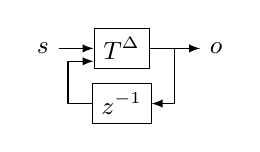
\begin{tikzpicture}[>=latex]
    \node[] (input) {$s$};
    \node[block, right of=input] (f) {$\inc{T}$};
    \node[right of=f, node distance=1.2cm] (output) {$o$};
    \node[block, below of=f, node distance=.7cm] (z) {$\zm$};
    \draw[->] (input) -- (f);
    \draw[->] (f) -- node (mid) {} (output);
    \draw[->] (mid.center) |-  (z);
    \draw[->] (z.west) -- ++(-.3,0) |- ([yshift=1mm]f.south west);
\end{tikzpicture}
\end{tabular}

In other words, the incremental version of a feedback loop around a query
is just the feedback loop with the incremental query for its body.  The significance
of this result will be apparent when we implement recursive queries.

To execute incremental queries efficiently, we want to compute directly
on streams of changes, without integrating them. The invariance property above shows
that stream operators $+$, $-$, and $\zm$ are identical to their incremental versions.
The following theorems generalize this to linear and bi-linear operators:

\begin{theorem}[Linear]\label{linear}
For an LTI operator $Q$ we have $\inc{Q}=Q$.
\end{theorem}

\begin{theorem}[Bilinear]\label{bilinear}
For a bilinear TI operator $\times$ we have
$\inc{(a \times b)} ~=~ a \times b ~+~ \zm(\I(a)) \times b ~+~ a \times \zm(\I(b))
= \I(a) \times b + a \times \zm(\I(b))$.
In pictures: \\
\noindent
\begin{tabular}{m{2.2cm}m{0cm}m{2.3cm}m{0cm}m{2.8cm}}
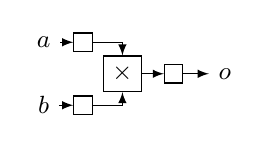
\begin{tikzpicture}[auto,node distance=.65cm,>=latex]
    \node[] (a) {$a$};
    \node[block, right of=a, node distance=.5cm] (ai) {$\I$};
    \node[below of=a, node distance=.4cm] (midway) {};
    \node[below of=midway, node distance=.4cm] (b) {$b$};
    \node[block, right of=b, node distance=.5cm] (bi) {$\I$};
    \node[block, right of=midway, node distance=1cm] (q) {$\times$};
    \node[block, right of=q] (D) {$\D$};
    \node[right of=D] (output) {$o$};
    \draw[->] (a) -- (ai);
    \draw[->] (b) -- (bi);
    \draw[->] (ai) -| (q);
    \draw[->] (bi) -| (q);
    \draw[->] (q) -- (D);
    \draw[->] (D) -- (output);
\end{tikzpicture} &
$\cong$ &
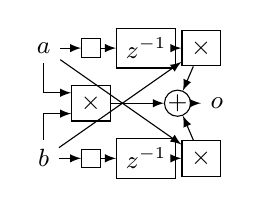
\begin{tikzpicture}[auto,>=latex,node distance=.7cm]
  \node[] (input1) {$a$};
  \node[below of=input1, node distance=1.4cm] (input2) {$b$};
  \node[block, right of=input1, node distance=.6cm] (I1) {$\I$};
  \node[block, below of=I1] (ab) {$\times$};
  \node[block, right of=input2, node distance=.6cm] (I2) {$\I$};
  \draw[->] (input1) -- (I1);
  \draw[->] (input2) -- (I2);
  \draw[->] (input1) |- ([yshift=-1mm]ab.north west);
  \draw[->] (input2) |- ([yshift=1mm]ab.south west);
  \node[block, right of=I1] (ZI1) {$\zm$};
  \node[block, right of=I2] (ZI2) {$\zm$};
  \draw[->] (I1) -- (ZI1);
  \draw[->] (I2) -- (ZI2);
  \node[block, right of=ZI1] (DI1) {$\times$};
  \node[block, right of=ZI2] (DI2) {$\times$};
  \draw[->] (ZI1) -- (DI1);
  \draw[->] (ZI2) -- (DI2);
  \node[block, circle, right of=ab, inner sep=0cm, node distance=1.1cm] (sum) {$+$};
  \draw[->] (ab) -- (sum);
  \draw[->] (DI1) -- (sum);
  \draw[->] (DI2) -- (sum);
  \node[right of=sum, node distance=.5cm] (output) {$o$};
  \draw[->] (sum) -- (output);
  \draw[->] (input1) -- (DI2);
  \draw[->] (input2) -- (DI1);
\end{tikzpicture}
&
$\cong$ &
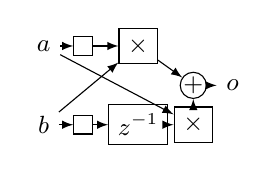
\begin{tikzpicture}[auto,>=latex,node distance=.7cm]
  \node[] (input1) {$a$};
  \node[below of=input1, node distance=1cm] (input2) {$b$};
  \node[block, right of=input1, node distance=.5cm] (I1) {$\I$};
  \node[block, right of=input2, node distance=.5cm] (I2) {$\I$};
  \draw[->] (input1) -- (I1);
  \draw[->] (input2) -- (I2);
  \node[block, right of=I2] (ZI2) {$\zm$};
  \draw[->] (I2) -- (ZI2);
  \node[block, right of=I1] (DI1) {$\times$};
  \node[block, right of=ZI2] (DI2) {$\times$};
  \draw[->] (I1) -- (DI1);
  \draw[->] (ZI2) -- (DI2);
  \node[block, circle, above of=DI2, inner sep=0cm, node distance=.5cm] (sum) {$+$};
  \draw[->] (DI1) -- (sum);
  \draw[->] (DI2) -- (sum);
  \node[right of=sum, node distance=.5cm] (output) {$o$};
  \draw[->] (sum) -- (output);
  \draw[->] (input1) -- (DI2);
  \draw[->] (input2) -- (DI1);
\end{tikzpicture}
\end{tabular}
\end{theorem}

If Theorem~\ref{bilinear} is rewritten using $\Delta a$ for the stream of changes to $a$ we
get the familiar formula for incremental equi-joins:
$\Delta(a\times b) =\Delta a \times \Delta b + a\times(\Delta b) + (\Delta a)\times b$; this is true because equi-joins are bilinear.

\section{IVM for the Relational Algebra}\label{sec:relational}

Results in \secref{sec:streams} and~\secref{sec:incremental}
apply to streams of arbitrary group values.  In this
section we use these results in the context of IVM for
relational databases.  As explained in the introduction, our goal is to
efficiently compute the incremental version of any relational query $Q$
that defines a database view.

However, we face a technical problem: the $\I$ and $\D$ operators were
defined on abelian groups, and relational databases in general are
not abelian groups, since they operate on sets.  Fortunately,
there is a well-known tool in the database literature
which converts set operations into group operations by using \zrs
(also called z-relations elsewhere~\cite{green-tcs11}) instead of sets.

We start by defining the \zrs group, and then we review how
relational queries are converted into \dbsp circuits  over \zrs.
This translation is efficiently incrementalizable because
many basic relational queries can be expressed using LTI \zr operators~\refsec{sec:relational-operators}.

\subsection{\zrs as an abelian group}

Given a set $A$, we define \defined{\zrs}
over $A$ as functions with \emph{finite support} from $A$ to $\Z$.
These are functions $f: A \rightarrow \Z$ where
$f(x) \not= 0$ for at most a finite number of values $x \in A$.
We also write $\Z[A]$ for the type of \zrs with elements from $A$.
Values in $\Z[A]$ can be thought of as key-value maps with
keys in $A$ and values in $\Z$, justifying the array indexing notation.
If $m \in \Z[A]$ we write $m[a]$ instead of $m(a)$, again using
an indexing notation.

A particular \zr $m \in \Z[A]$ can be denoted by enumerating its
elements that have non-zero values and their corresponding values:
$m = \{ x_1 \mapsto w_1, \dots, x_n \mapsto w_n \}$.
We call $w_i \in \Z$ the \defined{multiplicity} (or weight)
of $x_i \in A$.  Multiplicities can be negative.
We write that $x \in m$ iff $m[x] \not= 0$.
In terms of databases think of a \zr as a table
where each row as an associated weight, possibly negative.
We also write $w \cdot x$ for $\{ x \mapsto w \}$.

\ifzsetexamples
Consider a concrete \zr $R \in \Z[\texttt{string}]$,
defined by $R = \{ \texttt{joe} \mapsto 1, \texttt{anne} \mapsto -1 \}$.
$R$ has two elements in its domain,
\texttt{joe} with a multiplicity of 1 (so $R[\texttt{joe}] = 1$),
and \texttt{anne} with a multiplicity of $-1$.
We say \texttt{joe} $\in R$ and \texttt{anne} $\in R$.
\fi

Since $\Z$ is an abelian ring, $\Z[A]$ is also an abelian ring (and thus a group).  This group
$(\Z[A], +_{\Z[A]}, 0_{\Z[A]}, -_{\Z{A}})$ has addition and subtraction defined pointwise:
$(f +_{\Z[A]} g)(x) = f(x) + g(x) . \forall x \in A.$
The $0$ element of $\Z[A]$ is the function $0_{\Z[A]}$ defined by $0_{\Z[A]}(x) = 0 .
\forall x \in A$.  For example $R + R =  \{ \texttt{joe} \mapsto 2, \texttt{anne} \mapsto -2 \}$.
Since \zrs form a group, all the results from \secref{sec:streams} apply to streams over \zrs.

\zrs generalize sets and bags.  A set with elements from $A$
can be represented as a \zr by associating a weight of 1 with each element.
Bags are \zrs where all weights are positive.  Crucially, \zrs
can also represent arbitrary \emph{changes} to sets and bags.
Negative weights in a change represent elements that are being ``removed''.

\begin{definition}
We say that a \zr represents a \defined{set} if the multiplicity of every
element is one.  We define a function to check this property
$\isset : \Z[A] \rightarrow \B$\index{isset}
given by:
$$\isset(m) \defn \left\{
\begin{array}{ll}
  \mbox{true} & \mbox{ if } m[x] = 1, \forall x \in m \\
  \mbox{false} & \mbox{ otherwise}
\end{array}
\right.
$$
\end{definition}

\ifzsetexamples
For our example $\isset(R) = \mbox{false}$, since $R[\texttt{anne}] = -1$.
\fi

\begin{definition}
We say that a \zr is \defined{positive} (or a \defined{bag}) if the multiplicity of every element is
positive.  We define a function to check this property
$\ispositive : \Z[A] \rightarrow \B$\index{ispositive}.
given by
$$\ispositive(m) \defn \left\{
\begin{array}{ll}
  \mbox{true} & \mbox{ if } m[x] \geq 0, \forall x \in A \\
  \mbox{false} & \mbox{ otherwise}
\end{array}
\right.$$
$\forall m \in \Z[A] . \isset(m) \Rightarrow \ispositive(m)$.
\end{definition}

\ifzsetexamples
We have $\ispositive(R) = \mbox{false}$, since $R[\texttt{anne}] = -1$.
\fi

We write $m \geq 0$ when $m$ is
positive.  For positive $m, n$ we write $m \geq n$ for $m, n
\in \Z[A]$ iff $m - n \geq 0$.  $\geq$ is a partial order.

We call a function $f : \Z[A] \rightarrow \Z[B]$ \defined{positive} if it maps
positive values to positive values:
$\forall x \in \Z[A], x \geq 0_{\Z[A]} \Rightarrow f(x) \geq 0_{\Z[B]}$.
We apply this notation to functions as well: $\ispositive(f)$.

\begin{definition}[distinct]
The function $\distinct: \Z[A] \rightarrow \Z[A]$\index{distinct}
``converts'' a \zr into a set:
$$\distinct(m)[x] \defn \left\{
\begin{array}{ll}
  1 & \mbox{ if } m[x] > 0 \\
  0 & \mbox{ otherwise}
\end{array}
\right.
$$
\end{definition}

Notice that $\distinct$ ``removes'' duplicates from multisets, and it also eliminates
elements with negative multiplicities.
\ifzsetexamples
$\distinct(R) = \{ \texttt{joe} \mapsto 1 \}$.
\fi
While very simple, this definition of $\distinct$ has been carefully
chosen to enable us to implement the relational (set) operators
using \zrs operators.
%Circuits derived from relational queries only compute on positive \zrs.

%\begin{definition}(mononotonicity)
%A stream $s \in \stream{\Z[A]}$ is \defined{positive} if every value of the stream is positive:
%$s[t] \geq 0 . \forall t \in \N$.
%A stream $s \in \stream{\Z[A]}$ is \defined{monotone} if $s[t] \geq s[t-1], \forall t \in \N$.
%\end{definition}
%
%If $s \in \stream{\Z[A]}$ is positive, then $\I(s)$ is monotone.
%If $s \in \stream{\Z[A]}$ is monotone, $\D(s)$ is positive.
%
\paragraph{Generalizing circuit diagrams}

From now on we will use circuits to compute both on scalars (\zrs in our case) and streams of \zrs.
We use the same graphical representation for functions on streams or scalars:
boxes with input and output arrows.  For scalar functions the ``values''
of the arrows are scalars instead of streams; otherwise
the interpretation of boxes as function application is unchanged.  We will
thus use circuits to depict relational query plans.

\subsection{Implementing relational operators}\label{sec:relational-operators}

The fact that relational algebra can be implemented by computations
on \zrs has been shown before, e.g.~\cite{green-pods07}.  The translation
of the relational operators to \dbsp is shown in Table~\ref{tab:relational}.
The first row of the table shows that a composite query is translated
recursively.  This gives us a recipe for
translating an arbitrary relational query plan into a \dbsp circuit.

\newlength{\commentsize}
\setlength{\commentsize}{5cm}
\begin{table*}[h]
\small
\begin{tabular}{|m{1.2cm}m{4.2cm}m{5cm}m{\commentsize}|} \hline
Operation & SQL example & \dbsp circuit & Details \\ \hline
Composition &
 \begin{lstlisting}[language=SQL]
SELECT DISTINCT ... FROM
(SELECT ... FROM ...)
\end{lstlisting}
 &
 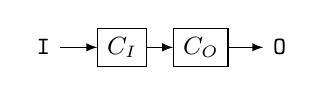
\begin{tikzpicture}[auto,>=latex]
  \node[] (I) {\code{I}};
  \node[block, right of=I] (CI) {$C_I$};
  \draw[->] (I) -- (CI);
  \node[block, right of=CI] (CO) {$C_O$};
  \node[right of=CO] (O) {\code{O}};
  \draw[->] (CI) -- (CO);
  \draw[->] (CO) -- (O);
\end{tikzpicture}
 &
 \parbox[b][][t]{\commentsize}{
  $C_I$ circuit for inner query, \\
  $C_O$ circuit for outer query.}
\\ \hline
Union &
\begin{lstlisting}[language=SQL]
(SELECT * FROM I1)
UNION
(SELECT * FROM I2)
\end{lstlisting}
&
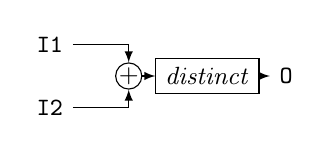
\begin{tikzpicture}[auto,>=latex]
  \node[] (input1) {\code{I1}};
  \node[below of=input1, node distance=.4cm] (midway) {};
  \node[below of=midway, node distance=.4cm] (input2) {\code{I2}};
  \node[block, shape=circle, right of=midway, inner sep=0in] (plus) {$+$};
  \node[block, right of=plus] (distinct) {$\distinct$};
  \node[right of=distinct] (output) {\code{O}};
  \draw[->] (input1) -| (plus);
  \draw[->] (input2) -| (plus);
  \draw[->] (plus) -- (distinct);
  \draw[->] (distinct) -- (output);
\end{tikzpicture}
&
\\ \hline
Projection &
\begin{lstlisting}[language=SQL]
SELECT DISTINCT I.c
FROM I
\end{lstlisting}
&
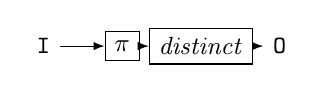
\begin{tikzpicture}[auto,>=latex]
  \node[] (input) {\code{I}};
  \node[block, right of=input] (pi) {$\pi$};
  \node[block, right of=pi] (distinct) {$\distinct$};
  \node[right of=distinct] (output) {\code{O}};
  \draw[->] (input) -- (pi);
  \draw[->] (pi) -- (distinct);
  \draw[->] (distinct) -- (output);
\end{tikzpicture}
&
\parbox[b][][t]{\commentsize}{
$\pi(i)[y] \defn
\sum_{x \in i, x|_c = y} i[x]$ \\
$x|_c$ is projection on column $c$ of the tuple $x$ \\
$\pi$ is linear; $\ispositive(\pi)$ %, \zpp{\pi}$.
}
\\ \hline
Filtering &
\begin{lstlisting}[language=SQL]
SELECT * FROM I
WHERE p(I.c)
\end{lstlisting}
&
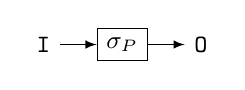
\begin{tikzpicture}[auto,>=latex]
  \node[] (input) {\code{I}};
  \node[block, right of=input] (map) {$\sigma_P$};
  \node[right of=map] (output) {\code{O}};
  \draw[->] (input) -- (map);
  \draw[->] (map) -- (output);
\end{tikzpicture}
&
\parbox[b][][t]{\commentsize}{
$\sigma_P(m)[x] \defn \left\{
\begin{array}{ll}
  m[x] \cdot x & \mbox{ if } P(x) \\
  0 & \mbox{ otherwise } \\
\end{array}
\right.$ \\
$P: A \rightarrow \B$ is a predicate. \\
$\sigma_P$ is linear; $\ispositive(\sigma_P)$ % \zpp{\sigma_P}$.
}
% \\ \hline
%Selection &
%\begin{lstlisting}[language=SQL]
%SELECT DISTINCT f(I.c, ...)
%FROM I
%\end{lstlisting}
%&
%\begin{tikzpicture}[auto,>=latex]
%  \node[] (input) {\code{I}};
%  \node[block, right of=input, node distance=1.5cm] (map) {$\mbox{map}(f)$};
%  \node[block, right of=map, node distance=1.5cm] (distinct) {$\distinct$};
%  \node[right of=distinct, node distance=1.5cm] (output) {\code{O}};
%  \draw[->] (input) -- (map);
%  \draw[->] (map) -- (distinct);
%  \draw[->] (distinct) -- (output);
%\end{tikzpicture}
%&
%\parbox[b][][t]{\commentsize}{
%For a function $f$ \\
%$\map(f)$ is linear, \\
%$\ispositive(\map(f)), \zpp{\map(f)}$
%}.
\\ \hline
\parbox[b][][t]{1cm}{
Cartesian \\
product} &
\begin{lstlisting}[language=SQL]
SELECT I1.*, I2.*
FROM I1, I2
\end{lstlisting}
&
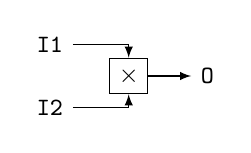
\begin{tikzpicture}[auto,>=latex]
  \node[] (i1) {\code{I1}};
  \node[below of=i1, node distance=.4cm] (midway) {};
  \node[below of=midway, node distance=.4cm] (i2) {\code{I2}};
  \node[block, right of=midway] (prod) {$\times$};
  \node[right of=prod] (output) {\code{O}};
  \draw[->] (i1) -| (prod);
  \draw[->] (i2) -| (prod);
  \draw[->] (prod) -- (output);
\end{tikzpicture}
&
\parbox[b][][t]{\commentsize}{
$(a \times b)((x,y)) \defn a[x] \times b[y]$. \\
$\times$ is bilinear, $\ispositive(\times)$ % , \zpp{\times}$.
}
\\ \hline
Equi-join &
\begin{lstlisting}[language=SQL]
SELECT I1.*, I2.*
FROM I1 JOIN I2
ON I1.c1 = I2.c2
\end{lstlisting}
&
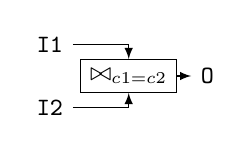
\begin{tikzpicture}[auto,>=latex]
  \node[] (i1) {\code{I1}};
  \node[below of=i1, node distance=.4cm] (midway) {};
  \node[below of=midway, node distance=.4cm] (i2) {\code{I2}};
  \node[block, right of=midway] (prod) {$\bowtie_{c1 = c2}$};
  \node[right of=prod] (output) {\code{O}};
  \draw[->] (i1) -| (prod);
  \draw[->] (i2) -| (prod);
  \draw[->] (prod) -- (output);
\end{tikzpicture}
&
\parbox[b][][t]{\commentsize}{
$(a \bowtie b)((x,y)) \defn a[x] \times b[y] \\
\mbox{ if } x|_{c1} = y|_{c2}$. \\
$\bowtie$ is bilinear, $\ispositive(\bowtie)$ %, \zpp{\bowtie}$.
}
\\ \hline
Intersection &
\begin{lstlisting}[language=SQL]
(SELECT * FROM I1)
INTERSECT
(SELECT * FROM I2)
\end{lstlisting}
&
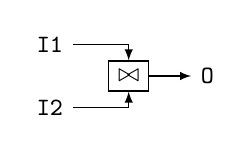
\begin{tikzpicture}[auto,>=latex]
  \node[] (i1) {\code{I1}};
  \node[below of=i1, node distance=.4cm] (midway) {};
  \node[below of=midway, node distance=.4cm] (i2) {\code{I2}};
  \node[block, right of=midway] (prod) {$\bowtie$};
  \node[right of=prod] (output) {\code{O}};
  \draw[->] (i1) -| (prod);
  \draw[->] (i2) -| (prod);
  \draw[->] (prod) -- (output);
\end{tikzpicture}
&
Special case of equi-join when both relations have the same schema.
 \\ \hline
Difference &
\begin{lstlisting}[language=SQL]
SELECT * FROM I1
EXCEPT
SELECT * FROM I2
\end{lstlisting}
&
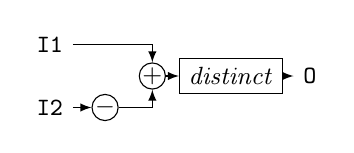
\begin{tikzpicture}[auto,>=latex, node distance=.7cm]
  \node[] (i1) {\code{I1}};
  \node[below of=i1, node distance=.4cm] (midway) {};
  \node[below of=midway, node distance=.4cm] (i2) {\code{I2}};
  \node[block, shape=circle, inner sep=0in, right of=i2] (m) {$-$};
  \node[block, right of=midway, shape=circle, inner sep=0in, node distance=1.3cm] (plus) {$+$};
  \node[block, right of=plus, node distance=1cm] (distinct) {$\distinct$};
  \node[right of=distinct, node distance=1cm] (output) {\code{O}};
  \draw[->] (i1) -| (plus);
  \draw[->] (i2) -- (m);
  \draw[->] (m) -| (plus);
  \draw[->] (plus) -- (distinct);
  \draw[->] (distinct) -- (output);
\end{tikzpicture}
&
\\ \hline
\end{tabular}
\caption{Implementation of SQL relational set operators in \dbsp.
Each query assumes that inputs \code{I}, \code{I1}, \code{I2}, are sets and it
produces output sets.\label{tab:relational}}
\end{table*}


The translation is fairly straightforward, but many operators require
the application of a $\distinct$ to produce sets.
For example, $a \cup b = \distinct(a + b)$, $a \setminus b =
\distinct(a - b)$, $(a \times b)((x,y)) = a[x] \times b[y]$.

%\paragraph{Correctness of the \dbsp implementations}\label{sec:correctness}
%
%A relational query $Q$ that transforms
%a set $V$ into a set $U$ is implemented by a \dbsp computation $Q'$ on
%\zrs.  The correctness of the implementation requires the following
%diagram to commute:
%
%\begin{center}
%\begin{tikzpicture}
%  \node[] (V) {$V$};
%  \node[below of=V] (VZ) {$VZ$};
%  \node[right of=V, node distance=2cm] (U) {$U$};
%  \node[below of=U] (UZ) {$UZ$};
%  \draw[->] (V) -- node (f) [below] {$Q$} (U);
%  \draw[->] (V) --  node (s) [left] {tozset}(VZ);
%  \draw[->] (VZ) -- node (f) [above] {$Q'$} (UZ);
%  \draw[->] (UZ) -- node (d) [right] {toset} (U);
%\end{tikzpicture}
%\end{center}
%
%(The correctness of
%this implementation is predicated on $Q'$'s inputs being
%sets, an invariant which needs to be maintained by the environment.)
%The ``$\mbox{toset}$'' and ``$\mbox{tozset}$'' functions convert sets to \zrs and
%vice-versa, in the expected way:
%
%$\mbox{toset}: \Z[A] \to 2^A$ is defined as $\mbox{toset}(m) \defn \cup_{x \in \distinct(m)} \{ x \}$.
%
%$\mbox{tozset}: 2^A \to \Z[A]$ is defined as $\mbox{tozset}(s) \defn \sum_{x \in s} 1 \cdot x$.

%All standard algebraic properties
%of the relational operators can be used to optimize circuits
%(they can even be applied to queries before building the circuits).

Notice that the use of the $\distinct$ operator allows \dbsp to model
the \emph{full relational algebra}, including set difference (and not
just the positive fragment).  Prior work (e.g., Proposition 6.13
in~\cite{green-tcs11}) has shown how some invocations of $\distinct$
can be eliminated from query plans without changing the query
semantics; we will see that each use of an incremental distinct incurs
significant space costs.

\begin{proposition}\label{prop-distinct-delay}
Let $Q$ be one of the following \zrs operators: filtering $\sigma$,
join $\bowtie$, or Cartesian product $\times$.
Then we have $\forall i \in \Z[I], \ispositive(i) \Rightarrow Q(\distinct(i)) = \distinct(Q(i))$.
\end{proposition}

\begin{comment}
\noindent
\begin{tabular}{m{3.5cm}m{.5cm}m{3.5cm}}
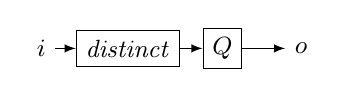
\begin{tikzpicture}[auto,>=latex]
  \node[] (input) {$i$};
  \node[block, right of=input, node distance=1.1cm] (distinct) {$\distinct$};
  \node[block, right of=distinct, node distance=1.2cm] (q) {$Q$};
  \node[right of=q] (output)  {$o$};
  \draw[->] (input) -- (distinct);
  \draw[->] (distinct) -- (q);
  \draw[->] (q) -- (output);
\end{tikzpicture}
&
$\cong$
&
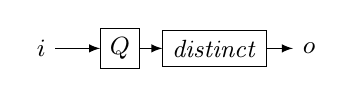
\begin{tikzpicture}[auto,>=latex]
  \node[] (input) {$i$};
  \node[block, right of=input] (q) {$Q$};
  \node[block, right of=q, node distance=1.2cm] (distinct1) {$\distinct$};
  \node[right of=distinct1, node distance=1.2cm] (output)  {$o$};
  \draw[->] (input) -- (q);
  \draw[->] (q) -- (distinct1);
  \draw[->] (distinct1) -- (output);
\end{tikzpicture}
\end{tabular}

This rule allows us to delay the application of $\distinct$.
\end{comment}

\begin{proposition}\label{prop-distinct-once}
Let $Q$ be one of the following \zrs operators: filtering $\sigma$,
projection $\pi$, map($f$)\footnote{Technically map (applying a user-defined
function to each row in a table) is not a relational operator.},
addition $+$, join $\bowtie$, or
Cartesian product $\times$.
Then we have $\ispositive(i) \Rightarrow \distinct(Q(\distinct(i))) = \distinct(Q(i))$.
\end{proposition}

\begin{comment}
\noindent
\begin{tabular}{m{6.5cm}m{.5cm}}
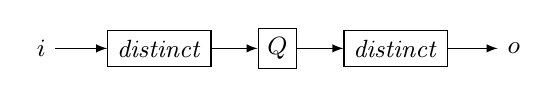
\begin{tikzpicture}[auto,>=latex]
  \node[] (input) {$i$};
  \node[block, right of=input, node distance=1.5cm] (distinct) {$\distinct$};
  \node[block, right of=distinct, node distance=1.5cm] (q) {$Q$};
  \node[block, right of=q, node distance=1.5cm] (distinct1) {$\distinct$};
  \node[right of=distinct1, node distance=1.5cm] (output)  {$o$};
  \draw[->] (input) -- (distinct);
  \draw[->] (distinct) -- (q);
  \draw[->] (q) -- (distinct1);
  \draw[->] (distinct1) -- (output);
\end{tikzpicture}
&
$\cong$ \\
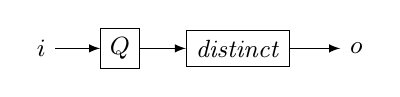
\begin{tikzpicture}[auto,>=latex]
  \node[] (input) {$i$};
  \node[block, right of=input] (q) {$Q$};
  \node[block, right of=q, node distance=1.5cm] (distinct1) {$\distinct$};
  \node[right of=distinct1, node distance=1.5cm] (output)  {$o$};
  \draw[->] (input) -- (q);
  \draw[->] (q) -- (distinct1);
  \draw[->] (distinct1) -- (output);
\end{tikzpicture}
\end{tabular}
\end{comment}

These properties allow us to ``consolidate'' distinct operators by performing
one $\distinct$ at the end of a chain of computations.

\subsection{Incremental view maintenance}

Let us consider a relational query $Q$
defining a view $V$.  To create a circuit that maintains incrementally $V$
we apply the following mechanical steps (this algorithm is deterministic
and its running time is proportional to the number of operators in the query):

\begin{algorithm}[incremental view maintenance]\label{algorithm-inc}\quad
\begin{enumerate}[nosep, leftmargin=\parindent]
    \item Translate $Q$ into a circuit using the rules in Table~\ref{tab:relational}.
    \item Apply $\distinct$ elimination rules (\ref{prop-distinct-delay}, \ref{prop-distinct-once}) until convergence\footnote{The
    order in which the rules are applied does not matter, since the algorithm is
    confluent: it always produces the same final result. So the rules can be applied in topological order.}.
    \item Lift the whole circuit, by applying Proposition~\ref{prop:distributivity},
    converting it to a circuit operating on streams.
    \item Incrementalize the whole circuit ``surrounding'' it with $\I$ and $\D$.
    \item Apply the chain rule
    from Proposition~\ref{prop-inc-properties} recursively on the query structure
    to obtain an incremental implementation.
\end{enumerate}
\end{algorithm}

A query can be implemented by multiple plans, with varying data-dependent costs.  The input provided
to this algorithm is a standard relational query plan, and this algorithm produces
an incremental plan that is ``similar'' to the input plan\footnote{Query planners generally use cost-based
heuristics to optimize plans, but IVM planning in general does not have this luxury, since the plan
must be generated \emph{before} the data has been fed to the database.  Nevertheless, standard query
optimization techniques, perhaps based on historical statistics, can be applied to the query plan before
generating the incremental plan.}.  Step (2) generates an equivalent circuit, with possibly
fewer $\distinct$ operators.
Step (3) yields a circuit that consumes a \emph{stream} of complete database snapshots and outputs a
stream of complete view snapshots. Step (4) yields a circuit that consumes a stream of \emph{database changes}
and outputs a stream of \emph{view changes}; however, the internal operation of the
circuit is non-incremental, as it rebuilds the complete database using
integration operators.  Step (5) incrementalizes the circuit by replacing each
primitive operators with its incremental version.

 Most of the operators that appear in the circuits in
Table~\ref{tab:relational} are linear, and thus have very efficient
incremental versions (we discuss complexity in \refsec{sec:complexity}).  A notable exception is $\distinct$.
The next proposition shows that the incremental version of $\distinct$
is also efficient, and it can be computed by doing work proportional to the size of the input change.

\begin{proposition}\label{prop-inc_distinct}
The following circuit implements $\inc{(\lift{\distinct})}$:
\begin{tabular}{m{3.5cm}m{.0cm}m{5cm}}
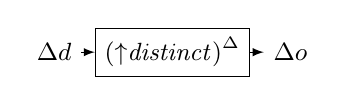
\begin{tikzpicture}[auto,node distance=1.5cm,>=latex]
    \node[] (input) {$\Delta d$};
    \node[block, right of=input] (d) {$\inc{(\lift{\distinct})}$};
    \node[right of=d] (output) {$\Delta o$};
    \draw[->] (input) -- (d);
    \draw[->] (d) -- (output);
\end{tikzpicture} &
$\cong$ &
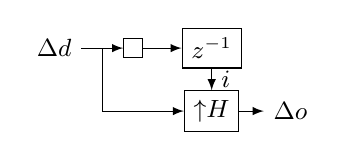
\begin{tikzpicture}[>=latex]
    \node[] (input) {$\Delta d$};
    \node[block, right of=input] (I) {$\I$};
    \node[block, right of=I] (z) {$\zm$};
    \node[block, below of=z, node distance=.8cm] (H) {$\lift{H}$};
    \node[right of=H] (output) {$\Delta o$};
    \draw[->] (input) -- node (mid) {} (I);
    \draw[->] (I) -- (z);
    \draw[->] (mid.center) |- (H);
    \draw[->] (z) -- node (i) [right] {$i$} (H);
    \draw[->] (H) -- (output);
\end{tikzpicture}
\end{tabular}

\noindent where $H: \Z[A] \times \Z[A] \to \Z[A]$ is defined as:
$$
H(i, d)[x] \defn
\begin{cases}
-1 & \mbox{if } i[x] > 0 \mbox{ and } (i + d)[x] \leq 0 \\
1  & \mbox{if } i[x] \leq 0 \mbox{ and } (i + d)[x] > 0 \\
0  & \mbox{otherwise} \\
\end{cases}
$$
\end{proposition}

Here is the intuition why $\distinct$ is efficiently
incrementalizable: the only elements that can appear in the output of
$\inc{(\lift{\distinct})}$ must have changed in the input.  So the
size of the output change cannot be bigger than the size of the input
change.  In the diagram above, $i$ is the previous version of the
integral of all changes, i.e., the full \zr whose $\distinct$ value is
being computed.  The function $H$ detects whether the multiplicity of
an element in $i$ is changing sign (positive to negative or
vice-versa) when adding a new delta $d$.

%\refsec{sec:relational-example} shows a concrete example of a relational query converted
%into a circuit and then incrementalized using Algorithm~\ref{algorithm-inc}.

\subsection{Complexity of incremental circuits}\label{sec:complexity}

Incremental circuits are efficient.  We evaluate the cost of a circuit
while processing the $t$-th input change.  We analyze cost from two
points of view: the work performed, and the total memory used.  Even
if $Q$ is a pure function, $\inc{Q}$ is actually a streaming system,
with internal state.  This state is stored entirely in the delay
operators $\zm$, some of which appear in $\I$ and $\D$ operators.  The
result produced by $\inc{Q}$ on the $t$-th input depends in general
not only on the new $t$-th input, but also on all prior inputs it has
received.

We argue that each operator in the incremental version of a circuit is
efficient in terms of work and space.  We make the standard IVM
assumption that the input changes \emph{of each operator} are small:
$|\Delta DB[t]| \ll |DB[t]| = |(\I(\Delta DB))[t]|$.

An unoptimized incremental operator $\inc{Q} = \D \circ Q \circ \I$
evaluates query $Q$ on the whole database $DB$, the integral of the input stream:
$DB = \I(\Delta DB)$; hence its time complexity  is the same as that of the non-incremental
evaluation of $Q$.  In addition, each of the $\I$ and $\D$ operators uses $O(|DB[t]|)$ memory.

Step (5) of the incrementalization algorithm applies the optimizations described in \secref{sec:incremental};
these reduce the time complexity of each operator to be a function of $O(|\Delta DB[t]|)$.
For example, Theorem~\ref{linear}, allows evaluating $\inc{S}$, where $S$ is a
linear operator, in time $O(|\Delta DB[t]|)$.  The $\I$
operator can also be evaluated in $O(|\Delta DB[t]|)$ time, because
all values that appear in the output of $\I(\Delta DB)[t]$ must be present in
current input change $\Delta DB[t]$.  Similarly, while the $\distinct$ operator is not
linear, $\inc{(\lift{\distinct})}$ can also be evaluated in $O(|\Delta DB[t]|)$ according to
Proposition~\ref{prop-inc_distinct}.  Bilinear operators, including join, can be
evaluated in time $O(|DB[t]| \times |\Delta DB[t]|)$, which is a factor of $|DB[t] / \Delta DB[t]|$
better than full re-evaluation.

The space complexity of linear operators is 0 (zero), since they store no
data persistently.  The space complexity of operators such as $\inc{(\lift{\distinct})}$,
$\inc{(\lift{\bowtie})}$, $\I$, and $\D$ is $O(|DB[t]|)$.

\subsection{Relational Query Example}\label{sec:relational-example}

We apply the IVM algorithm~\ref{algorithm-inc} to a concrete
relational SQL query:
\begin{lstlisting}[language=SQL,basicstyle=\small]
CREATE VIEW v AS
SELECT DISTINCT a.x, b.y FROM (
     SELECT t1.x, t1.id FROM t1 WHERE t1.a > 2
) a JOIN (
     SELECT t2.id, t2.y FROM t2 WHERE t2.s > 5
) b ON a.id = b.id
\end{lstlisting}

Step 1: Create a \dbsp circuit to represent this query using the
translation rules from Table~\ref{tab:relational}; notice that
this circuit is essentially a dataflow implementation of the query:

\noindent
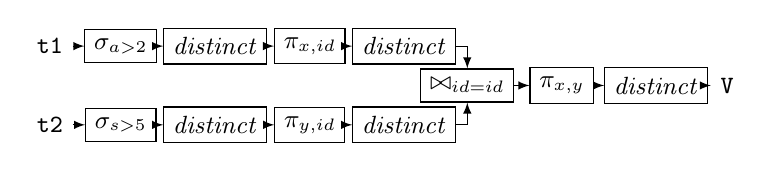
\begin{tikzpicture}[node distance=1.2cm,>=latex]
    \node[] (t1) {\code{t1}};
    \node[block, right of=t1, node distance=.9cm] (s1) {$\sigma_{a > 2}$};
    \node[block, right of=s1] (d1) {$\distinct$};
    \node[block, right of=d1] (p1) {$\pi_{x, id}$};
    \node[block, right of=p1] (d11) {$\distinct$};
    \node[below of=t1, node distance=1cm] (t2) {\code{t2}};
    \node[block, right of=t2, node distance=.9cm] (s2) {$\sigma_{s > 5}$};
    \node[block, right of=s2] (d2) {$\distinct$};
    \node[block, right of=d2] (p2) {$\pi_{y, id}$};
    \node[block, right of=p2] (d21) {$\distinct$};
    \node[below of=d11, node distance=.5cm] (mid) {};
    \node[block, right of=mid, node distance=.8cm] (j) {$\bowtie_{id = id}$};
    \node[block, right of=j] (p) {$\pi_{x, y}$};
    \node[block, right of=p] (d) {$\distinct$};
    \node[right of=d, node distance=.9cm] (V) {\code{V}};
    \draw[->] (t1) -- (s1);
    \draw[->] (s1) -- (d1);
    \draw[->] (d1) -- (p1);
    \draw[->] (p1) -- (d11);
    \draw[->] (t2) -- (s2);
    \draw[->] (s2) -- (d2);
    \draw[->] (d2) -- (p2);
    \draw[->] (p2) -- (d21);
    \draw[->] (d11) -| (j);
    \draw[->] (d21) -| (j);
    \draw[->] (j) -- (p);
    \draw[->] (p) -- (d);
    \draw[->] (d) -- (V);
\end{tikzpicture}

Step 2: apply the rules to eliminate $\distinct$ operators; first from
Proposition~\ref{prop-distinct-once}:

\noindent
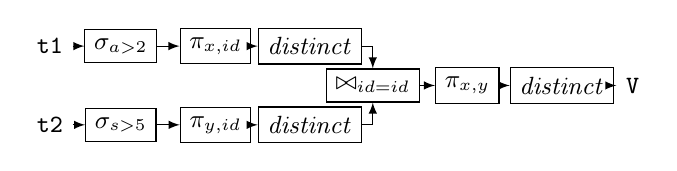
\begin{tikzpicture}[node distance=1.2cm,>=latex]
    \node[] (t1) {\code{t1}};
    \node[block, right of=t1, node distance=.9cm] (s1) {$\sigma_{a > 2}$};
    \node[block, right of=s1] (p1) {$\pi_{x, id}$};
    \node[block, right of=p1] (d11) {$\distinct$};
    \node[below of=t1, node distance=1cm] (t2) {\code{t2}};
    \node[block, right of=t2, node distance=.9cm] (s2) {$\sigma_{s > 5}$};
    \node[block, right of=s2] (p2) {$\pi_{y, id}$};
    \node[block, right of=p2] (d21) {$\distinct$};
    \node[below of=d11, node distance=.5cm] (mid) {};
    \node[block, right of=mid, node distance=.8cm] (j) {$\bowtie_{id = id}$};
    \node[block, right of=j] (p) {$\pi_{x, y}$};
    \node[block, right of=p] (d) {$\distinct$};
    \node[right of=d, node distance=.9cm] (V) {\code{V}};
    \draw[->] (t1) -- (s1);
    \draw[->] (s1) -- (p1);
    \draw[->] (p1) -- (d11);
    \draw[->] (t2) -- (s2);
    \draw[->] (s2) -- (p2);
    \draw[->] (p2) -- (d21);
    \draw[->] (d11) -| (j);
    \draw[->] (d21) -| (j);
    \draw[->] (j) -- (p);
    \draw[->] (p) -- (d);
    \draw[->] (d) -- (V);
\end{tikzpicture}

The rule from Proposition~\ref{prop-distinct-delay} gives:

\noindent
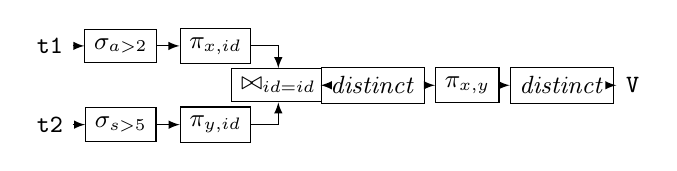
\begin{tikzpicture}[node distance=1.2cm,>=latex]
    \node[] (t1) {\code{t1}};
    \node[block, right of=t1, node distance=.9cm] (s1) {$\sigma_{a > 2}$};
    \node[block, right of=s1] (p1) {$\pi_{x, id}$};
    \node[below of=t1, node distance=1cm] (t2) {\code{t2}};
    \node[block, right of=t2, node distance=.9cm] (s2) {$\sigma_{s > 5}$};
    \node[block, right of=s2] (p2) {$\pi_{y, id}$};
    \node[below of=p1, node distance=.5cm] (mid) {};
    \node[block, right of=mid, node distance=.8cm] (j) {$\bowtie_{id = id}$};
    \node[block, right of=j] (d0) {$\distinct$};
    \node[block, right of=d0] (p) {$\pi_{x, y}$};
    \node[block, right of=p] (d) {$\distinct$};
    \node[right of=d, node distance=.9cm] (V) {\code{V}};
    \draw[->] (t1) -- (s1);
    \draw[->] (s1) -- (p1);
    \draw[->] (t2) -- (s2);
    \draw[->] (s2) -- (p2);
    \draw[->] (p1) -| (j);
    \draw[->] (p2) -| (j);
    \draw[->] (j) -- (d0);
    \draw[->] (d0) -- (p);
    \draw[->] (p) -- (d);
    \draw[->] (d) -- (V);
\end{tikzpicture}

Applying again~\ref{prop-distinct-once} we get:

\noindent
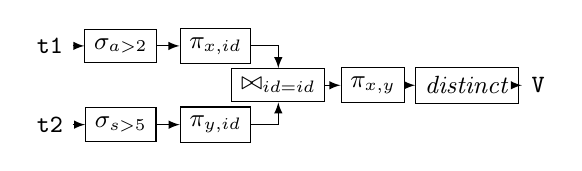
\begin{tikzpicture}[node distance=1.2cm,>=latex]
    \node[] (t1) {\code{t1}};
    \node[block, right of=t1, node distance=.9cm] (s1) {$\sigma_{a > 2}$};
    \node[block, right of=s1] (p1) {$\pi_{x, id}$};
    \node[below of=t1, node distance=1cm] (t2) {\code{t2}};
    \node[block, right of=t2, node distance=.9cm] (s2) {$\sigma_{s > 5}$};
    \node[block, right of=s2] (p2) {$\pi_{y, id}$};
    \node[below of=p1, node distance=.5cm] (mid) {};
    \node[block, right of=mid, node distance=.8cm] (j) {$\bowtie_{id = id}$};
    \node[block, right of=j] (p) {$\pi_{x, y}$};
    \node[block, right of=p] (d) {$\distinct$};
    \node[right of=d, node distance=.9cm] (V) {\code{V}};
    \draw[->] (t1) -- (s1);
    \draw[->] (s1) -- (p1);
    \draw[->] (t2) -- (s2);
    \draw[->] (s2) -- (p2);
    \draw[->] (p1) -| (j);
    \draw[->] (p2) -| (j);
    \draw[->] (j) -- (p);
    \draw[->] (p) -- (d);
    \draw[->] (d) -- (V);
\end{tikzpicture}

Step 3: we lift the circuit using distributivity (Proposition~\ref{prop:distributivity})
of composition over lifting; we
obtain a circuit that computes over streams, i.e., for each new input pair of relations
\code{t1} and \code{t2} it will produce an output view \code{V}:

\noindent
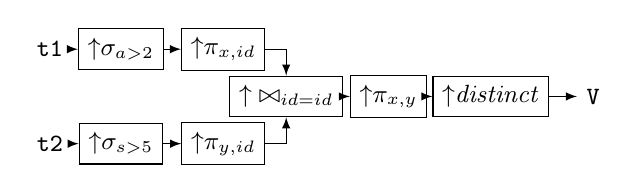
\begin{tikzpicture}[node distance=1.3cm,>=latex]
    \node[] (t1) {\code{t1}};
    \node[block, right of=t1, node distance=.9cm] (s1) {$\lift{\sigma_{a > 2}}$};
    \node[block, right of=s1] (p1) {$\lift{\pi_{x, id}}$};
    \node[below of=t1, node distance=1.2cm] (t2) {\code{t2}};
    \node[block, right of=t2, node distance=.9cm] (s2) {$\lift{\sigma_{s > 5}}$};
    \node[block, right of=s2] (p2) {$\lift{\pi_{y, id}}$};
    \node[below of=p1, node distance=.6cm] (mid) {};
    \node[block, right of=mid, node distance=.8cm] (j) {$\lift{\bowtie_{id = id}}$};
    \node[block, right of=j] (p) {$\lift{\pi_{x, y}}$};
    \node[block, right of=p] (d) {$\lift{\distinct}$};
    \node[right of=d] (V) {\code{V}};
    \draw[->] (t1) -- (s1);
    \draw[->] (s1) -- (p1);
    \draw[->] (t2) -- (s2);
    \draw[->] (s2) -- (p2);
    \draw[->] (p1) -| (j);
    \draw[->] (p2) -| (j);
    \draw[->] (j) -- (p);
    \draw[->] (p) -- (d);
    \draw[->] (d) -- (V);
\end{tikzpicture}

Step 4: incrementalize circuit, obtaining a circuit that computes over changes;
this circuit receives changes to relations \code{t1} and \code{t2} and for each
such change it produces the corresponding change in the output view \code{V}:

\noindent
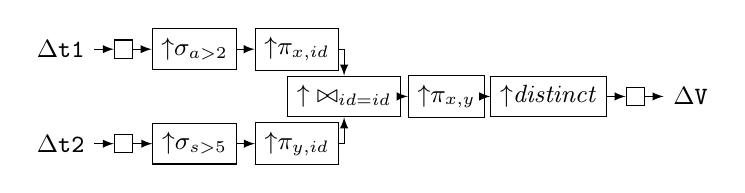
\begin{tikzpicture}[node distance=1.3cm,>=latex]
    \node[] (t1) {$\Delta$\code{t1}};
    \node[block, right of=t1, node distance=.8cm] (I1) {$\I$};
    \node[block, right of=I1, node distance=.9cm] (s1) {$\lift{\sigma_{a > 2}}$};
    \node[block, right of=s1] (p1) {$\lift{\pi_{x, id}}$};
    \node[below of=t1, node distance=1.2cm] (t2) {$\Delta$\code{t2}};
    \node[block, right of=t2, node distance=.8cm] (I2) {$\I$};
    \node[block, right of=I2, node distance=.9cm] (s2) {$\lift{\sigma_{s > 5}}$};
    \node[block, right of=s2] (p2) {$\lift{\pi_{y, id}}$};
    \node[below of=p1, node distance=.6cm] (mid) {};
    \node[block, right of=mid, node distance=.6cm] (j) {$\lift{\bowtie_{id = id}}$};
    \node[block, right of=j] (p) {$\lift{\pi_{x, y}}$};
    \node[block, right of=p] (d) {$\lift{\distinct}$};
    \node[block, right of=d, node distance=1.1cm] (D) {$\D$};
    \node[right of=D, node distance=.7cm] (V) {$\Delta$\code{V}};
    \draw[->] (t1) -- (I1);
    \draw[->] (I1) -- (s1);
    \draw[->] (s1) -- (p1);
    \draw[->] (t2) -- (I2);
    \draw[->] (I2) -- (s2);
    \draw[->] (s2) -- (p2);
    \draw[->] (p1) -| (j);
    \draw[->] (p2) -| (j);
    \draw[->] (j) -- (p);
    \draw[->] (p) -- (d);
    \draw[->] (d) -- (D);
    \draw[->] (D) -- (V);
\end{tikzpicture}

Step 5: apply the chain rule to rewrite the circuit as a composition of incremental operators;

\noindent
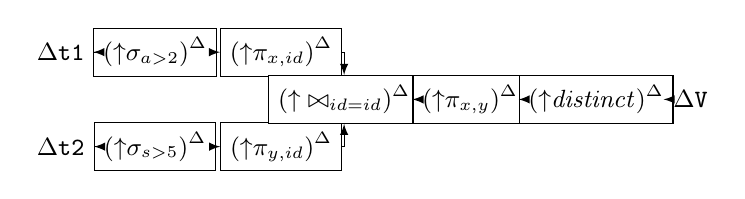
\begin{tikzpicture}[node distance=1.6cm,>=latex]
    \node[] (t1) {$\Delta$\code{t1}};
    \node[block, right of=t1, node distance=1.2cm] (s1) {$\inc{(\lift{\sigma_{a > 2}})}$};
    \node[block, right of=s1] (p1) {$\inc{(\lift{\pi_{x, id}})}$};
    \node[below of=t1, node distance=1.2cm] (t2) {$\Delta$\code{t2}};
    \node[block, right of=t2, node distance=1.2cm] (s2) {$\inc{(\lift{\sigma_{s > 5}})}$};
    \node[block, right of=s2] (p2) {$\inc{(\lift{\pi_{y, id}})}$};
    \node[below of=p1, node distance=.6cm] (mid) {};
    \node[block, right of=mid, node distance=.8cm] (j) {$\inc{(\lift{\bowtie_{id = id}})}$};
    \node[block, right of=j] (p) {$\inc{(\lift{\pi_{x, y}})}$};
    \node[block, right of=p] (d) {$\inc{(\lift{\distinct})}$};
    \node[right of=d, node distance=1.2cm] (V) {$\Delta$\code{V}};.8
    \draw[->] (t1) -- (s1);
    \draw[->] (s1) -- (p1);
    \draw[->] (t2) -- (s2);
    \draw[->] (s2) -- (p2);
    \draw[->] (p1) -| (j);
    \draw[->] (p2) -| (j);
    \draw[->] (j) -- (p);
    \draw[->] (p) -- (d);
    \draw[->] (d) -- (V);
\end{tikzpicture}

Use the linearity of $\sigma$ and $\pi$ to simplify this circuit (notice that
all linear operators no longer have a $\inc{\cdot}$):

\noindent
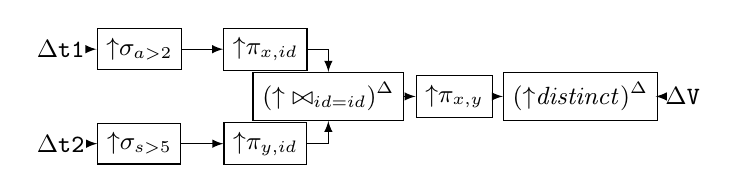
\begin{tikzpicture}[node distance=1.6cm,>=latex]
    \node[] (t1) {$\Delta$\code{t1}};
    \node[block, right of=t1, node distance=1cm] (s1) {$\lift{\sigma_{a > 2}}$};
    \node[block, right of=s1] (p1) {$\lift{\pi_{x, id}}$};
    \node[below of=t1, node distance=1.2cm] (t2) {$\Delta$\code{t2}};
    \node[block, right of=t2, node distance=1cm] (s2) {$\lift{\sigma_{s > 5}}$};
    \node[block, right of=s2] (p2) {$\lift{\pi_{y, id}}$};
    \node[below of=p1, node distance=.6cm] (mid) {};
    \node[block, right of=mid, node distance=.8cm] (j) {$\inc{(\lift{\bowtie_{id = id}})}$};
    \node[block, right of=j] (p) {$\lift{\pi_{x, y}}$};
    \node[block, right of=p] (d) {$\inc{(\lift{\distinct})}$};
    \node[right of=d, node distance=1.3cm] (V) {$\Delta$\code{V}};.8
    \draw[->] (t1) -- (s1);
    \draw[->] (s1) -- (p1);
    \draw[->] (t2) -- (s2);
    \draw[->] (s2) -- (p2);
    \draw[->] (p1) -| (j);
    \draw[->] (p2) -| (j);
    \draw[->] (j) -- (p);
    \draw[->] (p) -- (d);
    \draw[->] (d) -- (V);
\end{tikzpicture}

Finally, replace the incremental join using the formula for bilinear operators
(Theorem~\ref{bilinear}),
and the incremental $\distinct$ (Proposition~\ref{prop-inc_distinct}),
obtaining the following circuit (we omit the subscripts to save space):

\noindent
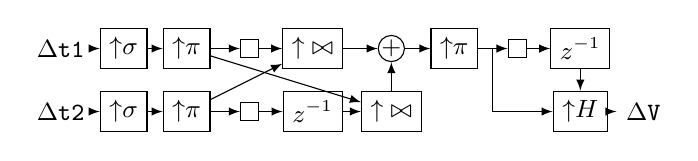
\begin{tikzpicture}[node distance=.8cm,>=latex]
    \node[] (t1) {$\Delta$\code{t1}};
    \node[block, right of=t1] (s1) {$\lift{\sigma}$};
    \node[block, right of=s1] (p1) {$\lift{\pi}$};
    \node[below of=t1, node distance=.8cm] (t2) {$\Delta$\code{t2}};
    \node[block, right of=t2] (s2) {$\lift{\sigma}$};
    \node[block, right of=s2] (p2) {$\lift{\pi}$};

    % join expansion
      \node[block, right of=p1] (jI1) {$\I$};
      \node[block, right of=p2] (jI2) {$\I$};
      \draw[->] (p1) -- (jI1);
      \draw[->] (p2) -- (jI2);
      \node[block, right of=jI2] (ZI2) {$\zm$};
      \draw[->] (jI2) -- (ZI2);
      \node[block, right of=jI1] (DI1) {$\lift\bowtie$};
      \node[block, right of=ZI2, node distance=1cm] (DI2) {$\lift\bowtie$};
      \draw[->] (jI1) -- (DI1);
      \draw[->] (ZI2) -- (DI2);
      \node[block, circle, above of=DI2, inner sep=0cm] (sum) {$+$};
      \draw[->] (DI1) -- (sum);
      \draw[->] (DI2) -- (sum);
      \draw[->] (p1) -- (DI2);
      \draw[->] (p2) -- (DI1);

    \node[block, right of=sum] (p) {$\lift{\pi}$};
    \draw[->] (sum) -- (p);
    \node[block, right of=p] (Id) {$\I$};
    \node[block, right of=Id] (zd) {$\zm$};
    \node[block, below of=zd] (H) {$\lift{H}$};
    \node[right of=H] (V) {$\Delta$\code{V}};
    \draw[->] (t1) -- (s1);
    \draw[->] (s1) -- (p1);
    \draw[->] (t2) -- (s2);
    \draw[->] (s2) -- (p2);
    \draw[->] (p) -- node (tapp) {} (Id);
    \draw[->] (Id) -- (zd);
    \draw[->] (zd) -- (H);
    \draw[->] (tapp.center) |- (H);
    \draw[->] (H) -- (V);
\end{tikzpicture}

Notice that the resulting circuit contains three integration
operations: two from the join, and one from the $\distinct$.  It also
contains two join operators.  However, the work performed by each
operator for each new input is proportional to the size of change.


\input{recursion}
\section{Incremental recursive programs}\label{sec:nested}

In \secref{sec:streams}--\ref{sec:relational} 
we showed how to incrementalize a relational query by
compiling it into a circuit, lifting the circuit to compute on streams, and
applying the $\inc{\cdot}$ operator.  In \secref{sec:recursion} we showed
how to compile a recursive query into a circuit that employs incremental
computation internally (using semi-na\"ive evaluation), to compute the fixed point.
Here we combine these results to construct a circuit that evaluates a \emph{recursive
query incrementally}.  The circuit receives a stream of updates to input
relations, and for every update recomputes the fixed point.  To do this
incrementally, it preserves the stream of changes to recursive relations
produced by the iterative fixed point computation, and adjusts this stream to
account for the modified inputs.  Thus, every element of the input stream yields
a stream of adjustments to the fixed point computation, using
\emph{nested streams}.

Nested streams, or streams of streams, $\stream{\stream{A}} = \N \rightarrow (\N
\rightarrow A)$, are well defined, since streams form an abelian group.
Equivalently, a nested stream is a value in $\N \times \N \to A$, i.e., a matrix
with an infinite number of rows, indexed by two-dimensional time $(t_0, t_1)$. 
where each row is a stream.  Please refer to our companion report for
example computations on nested streams~\cite{tr}.

%In the Appendix in
%\secref{sec:nested-examples} we show a few example nested stream
%computations.

Lifting a stream operator $S: \stream{A} \to \stream{B}$ yields an operator over
nested streams $\lift{S}: \stream{\stream{A}} \to \stream{\stream{B}}$, such
that $(\lift{S})(s) = S \circ s$, or, pointwise: $(\lift{S}(s))[t_0][t_1] =
S(s[t_0])[t_1], \forall t_0, t_1 \in \N$.  In particular, a scalar function $f:
A \rightarrow B$ can be lifted twice to produce an operator between streams of
streams: $\lift{\lift{f}}: \stream{\stream{A}} \rightarrow \stream{\stream{B}}$.

To define recursive nested queries, we need a slightly different definition of strictness. If we think of a nested stream $F: \stream{\stream{A}} \to \stream{\stream{B}}$ as a function of timestamps $(i, j)$, then the prior definition of strictness corresponds to strictness in the first dimension $i$, which we extend here to allow $F$ to be strict in its second dimension $j$: for any $s, s' \in \stream{\stream{A}}$ and all times $t \in \N$, $\forall i, j < t.\, s[i][j] = s'[i][j]$ implies $F(s)[i][t] = F(s')[i][t]$.
Proposition~\ref{prop-unique-fix} holds for this extended notion of strictness, i.e., the fixed point operator $\fix{\alpha}{F(\alpha)}$ is well defined for a strict operator $F$.

\begin{proposition}\label{prop-liftz}
The operator $\lift{\zm}: \stream{\stream{A}} \to \stream{\stream{A}}$ is strict (in its second dimension).
\end{proposition}

The operator $\zm$ on nested streams delays ``rows'' of the matrix, 
while $\lift{\zm}$ delays ``columns''.  
The $\I$ operator on $\stream{\stream{A}}$ operates on rows
of the matrix, treating each row as a single value.
Lifting a stream operator computing on $\stream{A}$, 
such as $\I: \stream{A} \to \stream{A}$, also produces an operator on nested streams, but
this time computing on the columns of the matrix
$\lift{\I}: \stream{\stream{A}} \to \stream{\stream{A}}.$  

\begin{proposition}[Lifting cycles]
\label{prop-lift-cycle}
For a binary, causal $T$ we have:
$\lift{(\lambda s. \fix{\alpha}{T(s,\zm(\alpha)}))} = \lambda s. \fix{\alpha}{(\lift{T})(s,(\lift{\zm})(\alpha))}$
\noindent i.e., lifting a circuit containing a ``cycle'' can be accomplished by
lifting all operators independently, including the $\zm$ back-edge.
\end{proposition}

This means that lifting a \dbsp stream operator can be expressed within \dbsp
itself.  For example, we have:

\begin{tabular}{m{2cm}m{.5cm}m{4cm}}
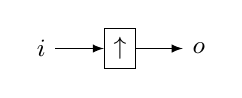
\begin{tikzpicture}[>=latex]
  \node[] (input) {$i$};
  \node[block, right of=input] (I) {$\lift{\I}$};
  \node[right of=I] (output)  {$o$};
  \draw[->] (input) -- (I);
  \draw[->] (I) -- (output);
\end{tikzpicture}
& $\cong$ &
\begin{tikzpicture}[>=latex]
  \node[] (input) {$i$};
  \node[block, circle, right of=input, inner sep=0cm] (p) {$+$};
  \node[right of=p, node distance=1.5cm] (output)  {$o$};
  \node[block, below of=p, node distance=.7cm] (z) {$\lift{\zm}$};
  \draw[->] (input) -- (p);
  \draw[->] (p) -- node (mid) {} (output);
  \draw[->] (z) -- (p);
  \draw[->] (mid.center) |- (z);
\end{tikzpicture}
\end{tabular}

This proposition gives the ability to lift
entire circuits, including circuits computing on streams and having feedback edges,
which are well-defined, due to Proposition~\ref{prop-liftz}.  
With this machinery we can now apply Algorithm~\ref{algorithm-inc} to arbitrary
circuits, even circuits built for recursively-defined relations.  

Step 1: Start with the ``semi-naive'' circuit~(\ref{eq:seminaive}):
\begin{center}
\begin{tikzpicture}[>=latex]
  \node[] (Iinput) {\code{I}};
  \node[block, right of=Iinput] (Idelta) {$\delta_0$};
  \node[block, right of=Idelta] (f) {$\inc{(\lift{R})}$};
  \node[block, right of=f, node distance=1.5cm] (S) {$\int$};
  \node[right of=S] (output)  {\code{O}};
  \draw[->] (f) -- node (o) {} (S);
  \node[block, below of=o, node distance=.7cm] (z) {$\zm$};
  \draw[->] (Iinput) -- (Idelta);
  \draw[->] (S) -- (output);
  \draw[->] (o.center) -- (z);
  \draw[->] (z) -| (f);
  \draw[->] (Idelta) -- (f);
\end{tikzpicture}
\vspace{-2mm}
\end{center}
\noindent Step 2: nothing to do (for $\distinct$). \\
\noindent Steps 3 and 4: Lift the circuit (using~\ref{prop-lift-cycle}) and incrementalize: \\
\begin{center}
\begin{tikzpicture}[>=latex]
  \node[] (Iinput) {$\Delta$\code{I}};
  \node[block, right of=Iinput] (I) {$\I$};
  \node[block, right of=I] (Idelta) {$\lift{\delta_0}$};
  \node[block, right of=Idelta, node distance=1.5cm] (f) {$\lift{\inc{(\lift{R})}}$};
  \node[block, right of=f, node distance=1.5cm] (S) {$\lift{\int}$};
  \node[block, right of=S] (D) {$\D$};
  \node[right of=D] (output)  {$\Delta$\code{O}};
  \draw[->] (f) -- node (o) {} (S);
  \node[block, below of=o, node distance=.7cm] (z) {$\lift{\zm}$};
  \draw[->] (Iinput) -- (I);
  \draw[->] (I) -- (Idelta);
  \draw[->] (S) -- (D);
  \draw[->] (D) -- (output);
  \draw[->] (o.center) -- (z);
  \draw[->] (z) -| (f);
  \draw[->] (Idelta) -- (f);
\end{tikzpicture}
\end{center}

\noindent Step 5: apply the chain rule and linearity of $\lift{\delta_0}$ and $\lift{\int}$:
\begin{equation}
\vspace{-2.1ex}
\begin{aligned}
\label{eq:increcursive}
\begin{tikzpicture}[>=latex]
  \node[] (Iinput) {$\Delta$\code{I}};
  \node[block, right of=Iinput] (Idelta) {$\lift{\delta_0}$};
  \node[block, right of=Idelta, node distance=2cm] (f) {$\inc{(\lift{\inc{(\lift{R})}})}$};
  \node[block, right of=f, node distance=2cm] (S) {$\lift{\int}$};
  \node[right of=S] (output)  {$\Delta$\code{O}};
  \draw[->] (f) -- node (o) {} (S);
  \node[block, below of=o, node distance=.7cm] (z) {$\lift{\zm}$};
  \draw[->] (Iinput) -- (Idelta);
  \draw[->] (S) -- (output);
  \draw[->] (o.center) -- (z);
  \draw[->] (z) -| (f);
  \draw[->] (Idelta) -- (f);
\end{tikzpicture}
\end{aligned}
\end{equation}

\vspace{1mm}
This is the incremental version of an arbitrary recursive query.  An example can be found in the TR~\cite{tr}.

%\refsec{sec:recursive-incremental-example} shows how Algorithm~\ref{algorithm-inc} is
%applied to the \dbsp circuit produced by the example from~\refsec{sec:recursive-example},
%which implements the recursive query computing the transitive closure of a graph.

\subsection{Cost of incremental recursive queries}

\paragraph{Time complexity}

The time complexity of an incremental recursive query can be estimated as a product of
the number of fixed point iterations and the complexity of each iteration. The
incrementalized circuit (\ref{eq:increcursive}) never performs more
iterations than the non-incremental circuit (\ref{eq:seminaive}):
once the non-incremental circuit reaches the fixed point, its output is constant, 
and the derivative of corresponding value in the incrementalized circuit becomes 0.

Moreover, the work performed by each operator in the incremental
circuit is asymptotically less than the non-incremental
one\footnote{Under the standard assumptions enumerated
in~\refsec{sec:complexity}.}.  A detailed analysis can be found in our
companion report~\cite{tr}.

%As a concrete example, consider a join in a recursive circuit.
%A non-incremental implementation is shown in the Appendix in 
%example~\ref{recursive-join}.  The incremental implementation
%of the same circuit is in circuit~\ref{join-expansion}, and contains
%4 join operators.  The work performed by the non-incremental join is $O(|DB|^2)$ for
%each iteration.  The size of the inputs of each of the joins in the incremental
%circuit is shown in \ref{sec:work}.  We notice that the four join operators
%perform work $O(|\Delta DB|^2)$, $O(|DB| |\Delta DB|)$, $(O|DB| |\Delta DB|)$,
%and $O(|DB|, 0)$ \leonid{strange notation} respectively (the last operator performs work only in the first iteration),
%so each of them is asymptotically better than the non-incremental version.

\paragraph{Space complexity} Integration ($\I$) and differentiation ($\D$) of a
stream $\Delta s \in \stream{\stream{A}}$ use memory proportional to
$\sum_{t_2}\sum_{t_1}|s[t_1][t_2]|$, i.e., the total size of changes
aggregated over columns of the matrix.  The unoptimized circuit integrates
and differentiates respectively inputs and outputs of the recursive program
fragment.  As we move $\I$ and $\D$ inside the circuit using the chain rule, we
additionally store changes to intermediate streams.  Effectively we cache results of 
fixed point iterations from earlier timestamps to update them efficiently as new input changes arrive.
Notice that space usage is proportional to the \emph{number of iterations of the inner loop} 
that computes the fixed-point.  
Fortunately, many recursive algorithms converge in a relatively small number of steps
(for example, transitive closure requires a number of steps  log(graph diameter).




\section{\dbsp and richer query languages}\label{sec:extensions}

The \dbsp language can express a richer class of streaming computations (both incremental and non-incremental)
than those covered so far. In this section we enumerate several important classes of
queries that can be implemented in \dbsp, and thus can be incrementalized using Algorithm~\ref{algorithm-inc}.

\subsection{Multisets and bags}

In \secref{sec:relational} we have shown how to implement the relational algebra on sets.
Some SQL queries however produce \emph{multisets}, e.g., \code{UNION ALL}.
Since \zrs generalize multisets and bags, it is trivial to implement query
operators on multisets, by just omitting $\distinct$ operator invocations.
For example, SQL \code{UNION} is \zr addition followed by $\distinct$,
whereas \code{UNION ALL} is just \zr addition.  Indeed, the SQL to \dbsp compiler
mentioned in \refsec{sec:implementation} handles full standard SQL, including
all multiset queries.

\subsection{Aggregation}\label{sec:aggregation}

Aggregation in SQL applies a function $a$ to a set of values of type $A$ producing a ``scalar''
result with some result type $B$: $a: 2^A \to B$.  In \dbsp an aggregation function has
a signature $a: \Z[A] \to B$.

The SQL \texttt{COUNT} aggregation function is implemented on \zrs by $a_\texttt{COUNT} : \Z[A] \to \Z$, which
computes a \emph{sum} of all the element weights: $a_\texttt{COUNT}(s) = \sum_{x \in s} s[x]$.
The SQL \texttt{SUM} aggregation function is implemented on \zrs by $a_\texttt{SUM}: \Z[\R] \to \R$ which
performs a \emph{weighted sum} of all (real) values: $a_\texttt{SUM}(s) = \sum_{x \in s} x \times s[x]$.
Both these implementations work correctly for sets and multisets.\footnote{If \texttt{COUNT DISTINCT} is needed,
the function would sum 1 for each element rather than its weight.}

With this definition the aggregation functions $a_\texttt{COUNT}$ and $a_\texttt{SUM}$ are in
fact linear transformations between the group $\Z[A]$ and the result group ($\Z$, and $\R$ respectively).

If the output of the \dbsp circuit is allowed to be such a ``scalar'' value, then aggregation
with a linear function is simply function application, and thus linear.
However, in general, composing multiple queries
requires the result of an aggregation to be a singleton \zr (containing a single value),
and not a scalar value.  In this case the aggregation function is implemented in
\dbsp as the composition of the actual aggregation and the
$\makeset: A \to \Z[A]$ function,
which converts a scalar value of type $A$ to a singleton \zr, defined as follows:
$\makeset(x) \defn \{ x \mapsto 1 \}$.

In conclusion, the following SQL query:
\code{SELECT SUM(c) FROM I}
is implemented as the following circuit:\footnote{The actual SQL \texttt{SUM} aggregate is
even more complicated, because it needs to skip \texttt{NULL}s,
and it returns \texttt{NULL} for an empty input set;
this behavior can be accurately implemented in \dbsp.}

\begin{tikzpicture}[auto,>=latex]
  \node[] (I) {\code{I}};
  \node[block, right of=I] (pi) {$\pi_\texttt{C}$};
  \node[block, right of=pi] (a) {$a_\texttt{SUM}$};
  \draw[->] (I) -- (pi);
  \draw[->] (pi) -- (a);
  \node[block, right of=a, node distance=1.5cm] (m) {$\makeset$};
  \node[right of=m] (O) {\code{O}};
  \draw[->] (a) -- (m);
  \draw[->] (m) -- (O);
\end{tikzpicture}

The lifted incremental version of this circuit is interesting: since $\pi$
and $a_\texttt{SUM}$ are linear, they are equivalent to their own incremental
versions.  Although $\inc{(\lift \makeset)} = \D \circ \lift{\makeset} \circ \I$
cannot be simplified, it is nevertheless efficient, doing only O(1) work per
invocation, since its input and output are singleton values.

%An aggregation function such as \texttt{AVG} can be written as the composition of
%a linear function that computes a pair of values using
%\texttt{SUM} and \texttt{COUNT}, followed by a division and a call to \makeset.

%\begin{lstlisting}[language=SQL]
%SELECT AVG(c) FROM I
%\end{lstlisting}
%
%\begin{tikzpicture}[auto,>=latex]
%  \node[] (I) {\code{I}};
%  \node[block, right of=I] (pi) {$\pi_\texttt{C}$};
%  \node[block, right of=pi, node distance=1.4cm] (sc) {$(a_\texttt{SUM}, a_\texttt{COUNT})$};
%  \draw[->] (I) -- (pi);
%  \draw[->] (pi) -- (sc);
%  \node[block, right of=sc, node distance=1.8cm] (m) {$\makeset$};
%  \node[block, right of=m, node distance=1.2cm] (div) {$\sigma_/$};
%  \node[right of=div] (O) {\code{O}};
%  \draw[->] (sc) -- (m);
%  \draw[->] (m) -- (div);
%  \draw[->] (div) -- (O);
%\end{tikzpicture}

Finally, some aggregate functions, such as \code{MIN}, are
\emph{not} linear: for handling deletions
they need to track the full set.  One way to implement in \dbsp the lifted
incremental version of such aggregate functions is
by ``brute force'', using the formula $\inc{(\lift a_\texttt{MIN})}
= \D \circ \lift{a_\texttt{MIN}} \circ \I$.  Such an implementations performs work
$O(|DB|)$ at each invocation.  However, schemes
such as Reactive Aggregator~\cite{tangwongsan-vldb15} can be implemented as custom \dbsp operators to bring
the amortized cost per update to $O(\log |DB|)$.  This approach is similar to the
customized implementation of the $\distinct$ operator, and it is another facet of
the modularity of \dbsp, which allows optimized operator implementations to be
mixed and matched, and can always fallback to brute-force.%
%\footnote{SQL's \code{ORDER BY} can also be modeled in \dbsp as
%a non-linear aggregate function that emits an ordered list.  However,
%such an implementation is not efficiently incrementalizable in \dbsp,
%doing $O(|DB|)$ work for every update.
%We leave the efficient handling of ORDER BY to future work.}

\subsection{Grouping; indexed relations}\label{sec:grouping}

Let $K$ be a set of ``key values.''
Consider the mathematical structure of finite maps from $K$
to \zrs: $K \to \Z[A] = \Z[A][K]$.
We call values $i$ of this structure \defined{indexed \zrs}: for
each key $k \in K$, $i[k]$ is a \zr.  Because
the codomain $\Z[A]$ is an abelian group, this structure is itself
an abelian group.

We use this structure to implement the SQL \texttt{GROUP BY} operator in \dbsp.
Consider a \defined{partitioning function}
$p: A \to K$ that assigns a key to any value in $A$.  We define the grouping function
$G_p: \Z[A] \to \Z[A][K]$ as $G_p(a)[k] \defn \sum_{x \in a.p(x)=k}a[x] \cdot x$
(just map each element of the input $a$ to the \zr grouping corresponding to its key).
When applied to a \zr $a$ this function returns a indexed \zr, where each element
is a \defined{grouping}:\footnote{We use
``group'' for the algebraic structure and ``grouping'' for the result of \code{GROUP BY}.} for each key $k$ a
grouping is a \zr containing all elements of $a$ that map to $k$
(as in SQL, groupings are multisets).
Consider our example \zr $R$ from \refsec{sec:relational},
and a key function $p(s)$ that returns the first letter of the string
$s$. Then we have that $G_p(R) = \{ \code{j} \mapsto \{ \code{joe}
\mapsto 1 \}, \code{a} \mapsto \{ \code{anne} \mapsto -1 \} \}$,
i.e., grouping with this key function produces an indexed \zr with two groupings, each
of which contains a \zr with one element.

The grouping function $G_p$ is linear for any key function $p$!
It follows that the group-by implementation in \dbsp is automatically
incremental: given some changes
to the input relation we can apply the partitioning function
to each change separately to compute how each grouping changes.

Notice that, unlike SQL, \dbsp can express naturally computations
on indexed \zrs, they are just an instance of a group structure.
In \dbsp one does not need to follow
grouping by aggregation, and \dbsp can represent nested groupings
of arbitrary depth.  Our definition of incremental
computation is only concerned with incrementality in the
\emph{outermost} structures.  We leave it to future work to
explore an appropriate definition of incremental computation
on the \emph{inner} relations.


\subsection{\texttt{GROUP BY-AGGREGATE}, flatmap}

Grouping in SQL is almost always followed by aggregation.
Let us consider an aggregation function $a: (K \times \Z[A]) \to B$ that produces values
in some group $B$, and an indexed relation of type $\Z[A][K]$, as defined above in~\refsec{sec:grouping}.
The nested relation aggregation operator $Agg_a: \Z[A][K] \to B$ applies $a$
to the contents of each grouping independently and adds the results:
$Agg_a(g) \defn \sum_{k \in K} a(k, g[k])$.  To apply this
to our example, let us compute the equivalent of \texttt{GROUP BY-COUNT}; we use
the following aggregation function $count: K \times \Z[A]$, $count(k, s) =
\makeset((k, a_\texttt{COUNT}(s)))$, using the \zr counting function $a_\texttt{COUNT}$
from~\refsec{sec:aggregation}; the notation $(a,b)$ is a pair of values $a$ and $b$.
Then we have $Agg_{count} (G_p(R)) = \{ (\code{j}, 1) \mapsto 1,
(\code{a}, -1) \mapsto 1 \}$.

%\subsection{\texttt{UNNEST} (flatmap)}

A very useful operation on nested relations is \defined{flatmap} (or \code{UNNEST} in SQL), which is
essentially the inverse of grouping, converting an indexed
\zr into a \zr: $\mbox{flatmap}: \Z[A][K] \to \Z[A \times K]$.
$\mbox{flatmap}$ is in fact a particular instance of aggregation,
using the aggregation function $a: K \times \Z[A] \to \Z[A \times K]$
defined by $a(k, s) = \sum_{x \in s[k]} s[k][x] \cdot (k, x).$
For our previous example, $\mbox{flatmap}(G_p(R)) = \{ (\code{j}, \code{joe}) \mapsto 1,
(\code{a}, \code{anne}) \mapsto -1 \}$.

%If we use an aggregation function $a: K \times Z[A]$ that is linear in its
%second argument, then the aggregation operator $Agg_a$ is linear, and
%thus fully incremental.  As a consequence, $\mbox{flatmap}$ is linear.
%However, many practical aggregation functions for nested relations are in fact
%not linear; an example is the $count$ function above, which is not linear
%since it uses the $\makeset$ non-linear function.  Nevertheless, while
%the incremental evaluation of such functions is not fully incremental,
%it is at least partly incremental: when applying a change to groupings, the aggregation
%function only needs to be re-evaluated \emph{for groupings that have changed}.

%\subsection{Antijoin}\label{sec:antijoin}\index{antijoin}
%
%Antijoins arise in the implementation of Datalog programs with stratified negation.
%Consider the following program:
%
%\begin{lstlisting}[language=ddlog,basicstyle=\small]
%O(v, z) :- I1(v, z), not I2(v).
%\end{lstlisting}
%
%The semantics of such a rule is defined in terms of joins and set difference.
%This rule is equivalent with the following pair of rules:
%
%\begin{lstlisting}[language=ddlog,basicstyle=\small]
%C(v, z) :- I1(v, z), I2(v).
%O(v, z) :- I1(v, z), not C(v, z).
%\end{lstlisting}
%
%This transformation reduces an antijoin to a join
%followed by a set difference.  This produces the following \dbsp circuit:
%
%\begin{tikzpicture}[auto,>=latex]
%  \node[] (i1) {\code{I1}};
%  \node[below of=i1, node distance=.5cm] (i2) {\code{I2}};
%  \node[block, right of=i1, node distance=1.5cm] (join) {$\bowtie$};
%  \node[block, shape=circle, inner sep=0in, right of=join] (m) {---};
%  \node[block, above of=m, shape=circle, inner sep=0in, node distance=.6cm] (plus) {$+$};
%  \node[block, right of=plus, node distance=1cm] (distinct) {$\distinct$};
%  \node[right of=distinct, node distance=1cm] (output) {\code{O}};
%  \draw[->] (i1) -- node (tap) {} (join);
%  \draw[->] (i2) -| (join);
%  \draw[->] (join) -- (m);
%  \draw[->] (m) -- (plus);
%  \draw[->] (tap.south) |- (plus);
%  \draw[->] (plus) -- (distinct);
%  \draw[->] (distinct) -- (output);
%\end{tikzpicture}
%
\subsection{Streaming joins}

Consider a binary query $T(s, t) = \I(s)~~\lift{\bowtie}~~t$.  This is the
\emph{relation-to-stream join} operator supported by streaming databases like Kafka's ksqlDB~\cite{jafarpour-edbt19}.
Stream $s$ carries changes to a relation, while $t$ carries arbitrary data, e.g., logs
or telemetry data points. $T$ discards values from $t$ after matching them against the accumulated contents of the relation $\I(s)$.

%\item[Explicit delay:]
%So far the $\zm$ operator was only used in integration or
%differentiation.  However, it can be exposed as a primitive operation that
%can be applied to streams.  This enables programs that can
%perform convolutions and time-based window computations over streams:

\paragraph{Streaming Window queries}

Streaming databases often organize the contents of streams into windows,
which store a subset of data points with a predefined range of timestamps.
%% The circuit below computes a \emph{fixed-size sliding-window aggregate}
%% over the last four timestamps with aggregations defined by the $T_i$ functions.
%%
%% \begin{center}
%% \begin{tikzpicture}[>=latex]
%%     \node[] (input) {$s$};
%%     \node[block, right of=input, node distance=1.5cm] (f0) {$T_0$};
%%     \node[below of=input, node distance=.5cm] (fake) {};
%%     \node[block, right of=fake, node distance=1cm] (z0) {$\zm$};
%%     \node[right of=input, node distance=.35cm] (tap) {};
%%     \node[block, right of=f0, node distance=1.5cm] (f1) {$T_1$};
%%     \node[block, right of=z0, node distance=1.2cm] (z1) {$\zm$};
%%     \node[block, right of=f1, node distance=1.5cm] (f2) {$T_2$};
%%     \node[block, right of=z1, node distance=1.5cm] (z2) {$\zm$};
%%     \draw[->] (input) -- (f0);
%%     \draw[->] (tap.center) |- (z0);
%%     \draw[->] (z0) -| (f0);
%%     \draw[->] (f0) -- (f1);
%%     \draw[->] (z0) -- (z1);
%%     \draw[->] (z1) -| (f1);
%%     \draw[->] (f1) -- (f2);
%%     \draw[->] (z1) -- (z2);
%%     \draw[->] (z2) -| (f2);
%%     \node[right of=f2] (output) {$o$};
%%     \draw[->] (f2) -- (output);
%% \end{tikzpicture}
%% \end{center}
%%
In practice, windowing is usually based on physical timestamps attached to
stream values rather than logical (transaction) time as in the previous circuit.
For instance, the CQL~\cite{arasu-tr02} query
``\texttt{SELECT * FROM events [RANGE 1 hour]}'' returns all events received
within the last hour.  The corresponding circuit (on the left)
takes input stream $s \in \stream{\Z[A]}$ and an additional
input $\theta \in \stream{\mathbb{R}}$ that carries the value of the current
time.

\begin{tabular}{m{3cm}m{0.5cm}m{3cm}}
\begin{tikzpicture}[>=latex]
    \node[] (input) {$s$};
    \node[above of=input, node distance=.5cm] (t) {$\theta$};
    \node[block, right of=input] (i) {$I$};
    \node[block, right of=i] (w) {$W$};
    \node[right of=w] (output) {$o$};
    \draw[->] (input) -- (i);
    \draw[->] (i) -- (w);
    \draw[->] (w) -- (output);
    \draw[->] (t) -| (w);
\end{tikzpicture}
&
$\cong$
&
\begin{tikzpicture}[>=latex]
    \node[] (input) {$s$};
    \node[above of=input, node distance=.5cm] (t) {$\theta$};
    \node[block, shape=circle, right of=input, inner sep=0pt] (plus) {$+$};
    \node[block, right of=plus] (w) {$W$};
    \node[right of=w] (output) {$o$};
    \node[block, below of=plus, node distance=.6cm] (z) {$\zm$};
    \draw[->] (input) -- (plus);
    \draw[->] (plus) -- (w);
    \draw[->] (t) -| (w);
    \draw[->] (w) -- node (mid) {} (output);
    \draw[->] (mid.center) |-  (z);
    \draw[->] (z) -- (plus);
\end{tikzpicture} \\
\end{tabular}

\noindent{}where the \emph{window operator} $W$ prunes input \zrs, only keeping values
with timestamps less than an hour behind $\theta[t]$.  Assuming $ts: A \to \mathbb{R}$ returns
the physical timestamp of a value, $W$ is defined as $W(v, \theta)[t] \defn \{x \in v[t] .
ts(x) \geq \theta[t] - 1hr\}$.  Assuming $\theta$ increases monotonically, $W$
can be moved inside integration, resulting in the circuit on the right, which uses
bounded memory to compute a window of an unbounded stream.
This circuit is a building block of a large family of window queries, including
window joins and window aggregation (e.g., SQL \texttt{OVER} queries).

\begin{comment}
\item[Weakening assumptions]

The theory as presented requires streams to be over group elements.  However,
this is necessary only if we want to automatically compute incremental
versions of the operators --- the addition and negation operations are
required for building $\I$ and $\D$.  The streaming circuits model
works very well on much simpler algebraic structures.  The $0$ element
is still needed to define $\zm$ and time-invariance.  Circuits that
mix streams over groups with arbitrary streams are well-defined.  However,
the zero-preservation property is required even for such general computations,
for the time-invariance of the resulting circuits.
\end{comment}

\begin{comment}
\item[Checkpoint/restore:]

The entire ``state'' of a streaming circuits is ``stored'' in its $\zm$ and $\lift{\zm}$
elements.  Saving this state amounts to taking a checkpoint of the streaming
system.  Restoring the state amounts to restoring a previous state.  These
operations can be the fundamental primitives for providing a fault-tolerant
implementation of a streaming query system.

\item[Materialized views:]

An incremental view maintenance system is not a database -- it only computes changes
to views when given changes to tables.  However, it can be integrated with a
database, by providing capabilities for \emph{querying} both tables and views.
An input table is just the integral of all the changes to the table.  This makes
possible building a system that is both stateful (like a database) and streaming
(like an incremental view maintenance system).
\end{comment}

\subsection{Relational while queries}

\dbsp can express programs that go beyond Datalog:
see the non-monotonic semantics for Datalog$^\neg$ and
Datalog$^{\neg\neg}$\cite{Abiteboul-book95}.
We implement the following
``while'' program, where $Q$ is an arbitrary query:
{\small
\begin{lstlisting}[language=Pascal]
x := i;
while (x changes)
    x := Q(x);
\end{lstlisting}}
The \dbsp implementation of this program is:

%$$\lambda i. \int[\D[\fix{\xi}{Q(\delta_0(i)+\zm(\xi))}]]$$
\begin{center}
\begin{tikzpicture}[>=latex]
  \node[] (input) {$i$};
  \node[block, right of=input] (delta) {$\delta_0$};
  \node[block, circle, right of=delta, inner sep=0cm] (p) {$+$};
  \node[block, right of=p] (Q) {$\lift Q$};
  \node[block, right of=Q] (D) {$\D$};
  \node[block, right of=D] (S) {$\int$};
  \node[right of=S] (output)  {$x$};
  \node[block, below of=p, node distance=.7cm] (z) {$\zm$};
  \draw[->] (input) -- (delta);
  \draw[->] (delta) -- (p);
  \draw[->] (p) -- (Q);
  \draw[->] (Q) -- node (mid) {} (D);
  \draw[->] (D) -- (S);
  \draw[->] (mid.center) |- (z);
  \draw[->] (S) -- (output);
  \draw[->] (z) -- (p);
\end{tikzpicture}
\end{center}

This circuit can be converted to a streaming circuit that computes a stream of values $i$
by lifting it; it can be incrementalized using Algorithm~\ref{algorithm-inc} to compute on changes of $i$:

\begin{center}
\begin{tikzpicture}[>=latex]
  \node[] (input) {$\Delta i$};
  \node[block, right of=input] (delta) {$\lift{\delta_0}$};
  \node[block, circle, right of=delta, inner sep=0cm] (p) {$+$};
  \node[block, right of=p] (Q) {$\inc{(\lift{\lift{Q}})}$};
  \node[block, right of=Q, node distance=1.5cm] (D) {$\lift{\D}$};
  \node[block, right of=D, node distance=1.1cm] (S) {$\lift{\int}$};
  \node[right of=S, node distance=1.2cm] (output)  {$\Delta x$};
  \node[block, below of=p, node distance=.7cm] (z) {$\lift{\zm}$};
  \draw[->] (input) -- (delta);
  \draw[->] (delta) -- (p);
  \draw[->] (p) -- (Q);
  \draw[->] (Q) -- node (mid) {} (D);
  \draw[->] (D) -- (S);
  \draw[->] (mid.center) |- (z);
  \draw[->] (S) -- (output);
  \draw[->] (z) -- (p);
\end{tikzpicture}
\end{center}

At runtime the execution of this circuit is not guaranteed to terminate;
however, if the circuit does terminate, it will produce the correct
output, i.e., the least fixpoint of $Q$ that includes~$i$.

\section{Implementation}\label{sec:implementation}

The scope of this paper is the \dbsp theory of IVM, so we only briefly touch upon
the implementation aspects.  We defer a full description and evaluation of the
system to a future paper.

\paragraph{\dbsp Rust library}

We have built an implementation of \dbsp as part of an
open-source project with an MIT license:
\anonymize{\url{https://github.com/vmware/database-stream-processor}}.
The implementation consists of a Rust library and a runtime.
The library provides APIs for basic algebraic data types:
such as groups, finite maps, \zr, indexed \zr.
A separate circuit construction API allows users to
create \dbsp circuits by placing operator nodes (corresponding to boxes in our diagrams)
and connecting them with streams, which correspond to the
arrows in our diagrams.  The library provides pre-built generic operators
for integration, differentiation, delay, nested integration and differentiation,
and a rich library of \zr basic incremental operators:
corresponding to plus, negation, grouping, joining, aggregation, $\distinct$,
flatmap, window aggregates, etc.

For iterative computations the library provides the $\delta_0$ operator and
an operator that approximates $\int$ by terminating iteration of
a loop at a user-specified condition (usually the condition is the
requirement for a zero to appear in a specified stream).
The low level library allows users to construct incremental
circuits manually by stitching together incremental versions of primitive operators.

The library supports data-parallel multicore evaluation of circuits
using a natural sharding strategy, and a variety of adapters for
external data sources (e.g., Kafka, CSV files, etc).  The library can
also spill internal operator state to persistent storage.  Benchmark
results (which are very promising) are available in the code
repository and will be discussed in future work.

\paragraph{SQL compiler}

We have also built a SQL to \dbsp compiler, which translates standard SQL queries
into \dbsp circuits.  The compiler implements Algorithm~\ref{algorithm-inc}, to
generate a streaming version of any SQL query.
The compiler is  open-source
\anonymize{\url{https://github.com/vmware/sql-to-dbsp-compiler}}
with an MIT license.  The compiler front-end parser and optimizer
are based on the Apache Calcite~\cite{begoli-icmd18} infrastructure.  The
project is mature enough to pass all 7 million SQL Logic Tests~\cite{sqllogictest}.  The compiler handles
all aspects of SQL, including NULLs, ternary logic, grouping, aggregation, multiset queries, etc.

\paragraph{Formal verification}

We have formalized and verified all the definitions, lemmas,
propositions, theorems, and examples in this paper using the Lean theorem prover; we make
these proofs available at~\anonymize{\cite{dbsp-theory}}.
% This amounted to roughly 5K lines of Lean code.
The formalization builds on mathlib~\cite{mathlib2020}, which provides
support for groups and functions with finite support (modeling
\zrs). We believe the simplicity of \dbsp enabled completing these
proofs in relatively few lines of Lean code (5K) and keeping a close
correspondence between the paper proofs in~\cite{tr} and Lean.

\input{related}
\section{Conclusions}\label{sec:conclusions}%\label{sec:ddlog}

We have introduced \dbsp, a model of computation based on infinite
streams over abelian groups.  In this model streams are used for 3
purposes: (1) to model consecutive snapshots of a database, (2) to
model consecutive changes (deltas, or transactions) applied to a
database and changes of a maintained view, (3) to model consecutive
values of loop-carried variables in recursive computations.

We have defined an abstract notion of incremental computation over
streams, and defined the incrementalization operator $\inc{\cdot}$,
which transforms an \emph{arbitrary} stream computation $Q$ into its
incremental version $\inc{Q}$.  The incrementalization operator has
some very nice algebraic properties, which gave us a general algorithm
for incrementalizing many classes of complex queries, including
arbitrary recursive queries.

We believe that \dbsp can form a solid foundation for a theory and practice of
streaming incremental computation.


\bibliographystyle{ACM-Reference-Format}
\bibliography{main}

%\appendix
%\input{appendix}

\end{document}
